
\definecolor{tableheader}{rgb}{0.8, 0.8, 0.8}
\definecolor{tableevenrow}{rgb}{0.95, 0.95, 0.95}
\definecolor{tableoddrow}{rgb}{1.0, 1.0, 1.0}

%----------------------------------------------------------------------------------------
\chapter{Contesto lavorativo}
\label{cap:introduzione}
\section{Profilo aziendale} \label{sec:azienda}
Zero12 s.r.l. è una \textit{startup} italiana fondata nel 2012, con attualmente due sedi operative: una a Padova (dove ho svolto lo \textit{stage}) e una ad Empoli. 
L'azienda è \textit{partner} \gls{awsg}, una piattaforma di servizi \textit{cloud} offerta da Amazon, ed è specializzata nello sviluppo di soluzioni \textit{cloud native}, offrendo ai propri clienti, proveniente da ambiti diversificati, soluzioni flessibili e scalibili. 
Ogni progetto viene svolto in tutte le sue parti dal \textit{team} di Zero12, dalla progettazione fino al suo sviluppo.
L’azienda è parte di Var Group S.p.A., l'operatore \textit{leader} nel settore dei servizi e delle soluzioni digitali. Supporta le imprese nel loro percorso di trasformazione digitale, offrendo ai propri \textit{partner} servizi e competenze per lo sviluppo di soluzioni innovative.
\section{Organizzazione aziendale}
Durante il mio periodo di \textit{stage} ho avuto modo osservare in prima persona l'organizzazione in \textit{team} di lavoro che l'azienda adotta.\\
Ho rappresentato di seguito nella tabella \ref{tab:ruoli} i ruoli che ho potuto osservare.
\renewcommand{\arraystretch}{1.5}
\begin{longtable}{|p{3.5cm}|p{8.7cm}|}
    \hline
    \rowcolor{tableheader}\textbf{Ruolo} & \textbf{Descrizione} \\
    \hline
    \endfirsthead

    \rowcolor{tableheader}\textbf{Ruolo} & \textbf{Descrizione} \\
    \hline
    \endhead

    \hline
    \endfoot

    \hline
    \endlastfoot
    \hline
    \rowcolor{tableoddrow}\textbf{\textit{CEO}} & Il \gls{ceog} ovvero l'amministratore delegato, rappresenta il ruolo più alto all'interno di una societa. Si occupa di definire le decisioni più importanti dell'azienda, di supervisionare i processi aziendali e di gestire i contatti con potenziali nuovi clienti. \\
    \hline
    \rowcolor{tableevenrow}\textbf{\textit{Project manager}} & Il \textit{project manager} è la figura che si occupa di gestire il progetto in tutte le sue fasi, di coordinare il \textit{team} di lavoro e di controllare che il progetto rispetti i costi, i tempi e le aspettative del cliente.\\
    \hline
    \rowcolor{tableoddrow}\textbf{\textit{Software developer}} & Il \textit{software developer} è la figura che si occupa della progettazione e dello sviluppo delle varie componenti \textit{software} individuate durante l'attività di analisi. Ognuno di loro si specializza nello sviluppo di funzionalità di \textit{frontend}, \textit{backend} o entrambi (\textit{fullstack})\\
    \hline
    \rowcolor{tableevenrow}\textbf{\textit{Mobile developer}} & Il \textit{mobile developer} è la figura che si occupa delle stesse mansioni del \textit{software developer}, riguardante un'applicativo \textit{mobile}. Nel contesto aziendale i \textit{mobile developers} si suddividono in due categorie: \textit{Android developers} e \textit{iOS developers}.\\
    \hline
    \rowcolor{tableoddrow}\textbf{\textit{AWS specialist}} & L'\textit{AWS Specialist} è la figura specializzata nella configurazione, gestione e adozione dei servizi offerti da \gls{aws}.\\
    \hline
    \rowcolor{tableevenrow}\textbf{\textit{HR}} & La figura dell' \gls{hrg} è una figura che si occupa della gestione delle risorse umane all'interno dell'azienda.\\
    \hline
    \caption{Organizzazione dei ruoli all'interno di Zero12 s.r.l.}
    \label{tab:ruoli}
\end{longtable}

\noindent
Ad ogni nuovo progetto viene assegnato un \textit{team} di lavoro composto da un \textit{project manager}, un numero variabile di \textit{software developers} o \textit{mobile developers}, a seconda delle esigenze del progetto, e un \textit{AWS specialist} se il progetto prevede l'utilizzo di servizi \gls{aws}. 

\section{Servizi e prodotti}
Zero12 offre vari servizi e prodotti che vengono richiesti dai propri clienti, provenienti da diversi ambiti.
Di seguito mostro una panoramica di tali servizi e prodotti offerti:
\begin{itemize}
    \item \textbf{\gls{aws} \textit{professional services}}: sin dalla sua nascita nel 2012, l'azienda propone e sviluppa soluzioni che sfruttano il \textit{cloud} e i servizi \gls{aws}. Per questo motivo, l'azienda mette a disposizione le competenze dei suoi specialisti
    per supportare i clienti nella migrazione verso il \textit{cloud} e nell'adozione dei servizi \gls{aws}.
    \item \textbf{Sviluppo di \textit{software custom}}: questo è un altro servizio offerto da Zero12. L'azienda si occupa della progettazione e dello sviluppo di \textit{software custom} (applicazioni \textit{web} e \textit{mobile}), adattandosi alle richieste ed alle esigenze del cliente. Il mio \textit{stage} ha seguito questa tipologia di progetto in cui l'azienda stessa era il cliente.
    \item \textbf{\textit{Machine learning}}: le soluzioni di \textit{machine learning} che Zero12 offre consistono nella creazione di modelli per l'analisi di linguaggio naturale, analisi di immagini e video, creati su misura secondo le esigenze del cliente.
    \item \textbf{\textit{Innovation advisory}}: servizio offerto progettato per trasformare le idee dei propri clienti in servizi digitali innovativi, sfruttando al massimo le potenzialità delle tecnologie \textit{cloud}. Questo servizio consente di sviluppare 
    soluzioni innovative e scalabili, adattabili alle esigenze del cliente.
\end{itemize}
\section{Processi aziendali}
\subsection{Metodologia di sviluppo}
Durante il mio periodo di \textit{stage} ho avuto modo di sperimentare in prima persona i processi istanziati dall'azienda per la realizzazione di un progetto.
La metodologia adottata dall'azienda è quella \textit{Agile}, adattandosi in particolare al \textit{framework Scrum}.
Ogni progetto viene suddiviso in \textit{sprint} di durata fissa e ad ognuno viene assegnato un \textit{team} di lavoro.
Nel contesto del mio \textit{stage}, la durata degli \textit{sprint} era di una settimana e il \textit{team} di lavoro era composta da me e dal mio \textit{tutor} aziendale.
Il ruolo che ho ricoperto all'interno del \textit{team} era quello di \textit{software developer}, mentre il mio \textit{tutor} ricopriva il ruolo di \textit{project manager}.
\begin{figure}[H]
    \centering
    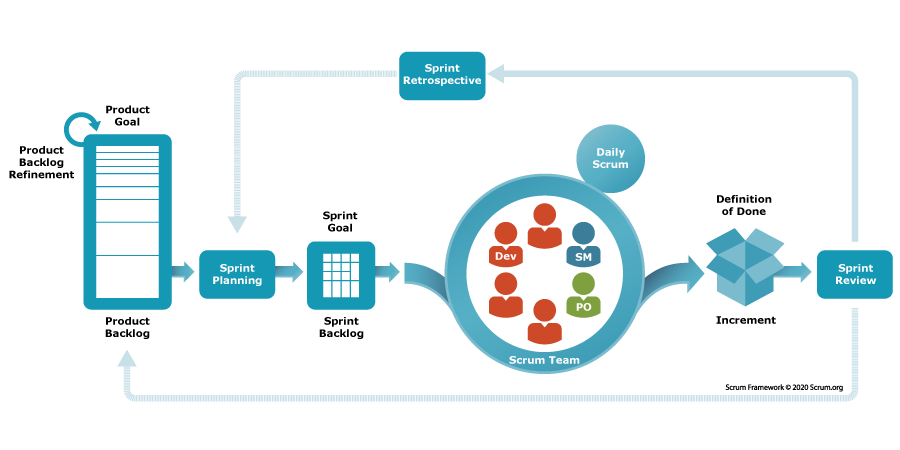
\includegraphics[width=0.8\textwidth]{scrum.png}
    \caption{Schema di flusso di un progetto con metodologia \textit{Scrum}}
    \small \textbf{Fonte:} \url{scrum.org}
    \label{fig:scrum}
\end{figure}
\noindent
La figura \ref{fig:scrum} mostra il flusso di lavoro di un progetto con metodologia \textit{Scrum} adottato da Zero12. Ogni nuovo progetto segue questo flusso. 
\begin{itemize}
    \item \textit{\gls{User-stories}}: all'inizio viene effettuata una prima sessione di \textit{user stories mapping} che va a definire quello che sarà presente nel \textit{product backlog}. Questa sessione viene svolta insieme al cliente, in modo da avere una chiara visione delle aspettative del cliente, definendo cosi anche, le \textit{feature} più importanti da sviluppare.
    \item \textbf{\textit{Sprint planning}}: all'inizio di ogni \textit{sprint} vengono selezionate le \textit{task} da svolgere, in base alla priorità, dal \textit{product backlog} e vengono assegnate ai membri del \textit{team} di lavoro. Gli \textit{sprint} hanno una durata di una o due settimane.
    \item \textbf{\textit{Daily stand-up}}: ogni giorno, ad un orario prefissato, il \textit{team} di lavoro si riunisce per discutere come procede il lavoro, cosa è stato fatto il giorno precedente e cosa verrà svolto durante la giornata. Hanno una durata di circa 15 minuti.
    \item \textbf{\textit{Sprint review}}: alla fine di ogni \textit{sprint} viene effettuata una revisione del lavoro svolto, andando a controllare che le \textit{task} assegnate siano completate e che il lavoro assegnato sia stato svolto in modo conforme alle aspettative del cliente.
    \item \textbf{\textit{Sprint retrospective}}: alla fine di ogni \textit{sprint} viene effettuato un controllo interno del lavoro svolto durante lo \textit{sprint}, andando ad evidenziare eventuali problematiche sorte e andando a definire eventuali miglioramenti da apportare al processo di lavoro.
\end{itemize}
\subsection{Strumenti di supporto ai processi}
\subsubsection{Jira}
\textit{Jira} è un \gls{itsg} che permette la gestione delle \textit{task} dei progetti in modo \textit{Agile}. All'inizio di ogni \textit{sprint}, lo \textit{scrum master} crea una nuova \textit{board} relativa allo \textit{sprint} in corso e assegna le \textit{task} (crea i \textit{ticket}) da svolgere ai membri del \textit{team} di lavoro.
I membri del \textit{team} di lavoro possono notificare lo stato del \textit{ticket}, spostandolo tra le varie colonne quali: 
\begin{itemize}
    \item \textbf{Da completare}: \textit{ticket} assegnati ma che devono essere ancora completati.
    \item \textbf{In corso}: \textit{ticket} assegnati ad una o più risorse del \textit{team} di lavoro e che sono in sviluppo.
    \item \textbf{Completato}: \textit{ticket} completati e pronti per la revisione.
\end{itemize}
\begin{figure}[H]
    \centering
    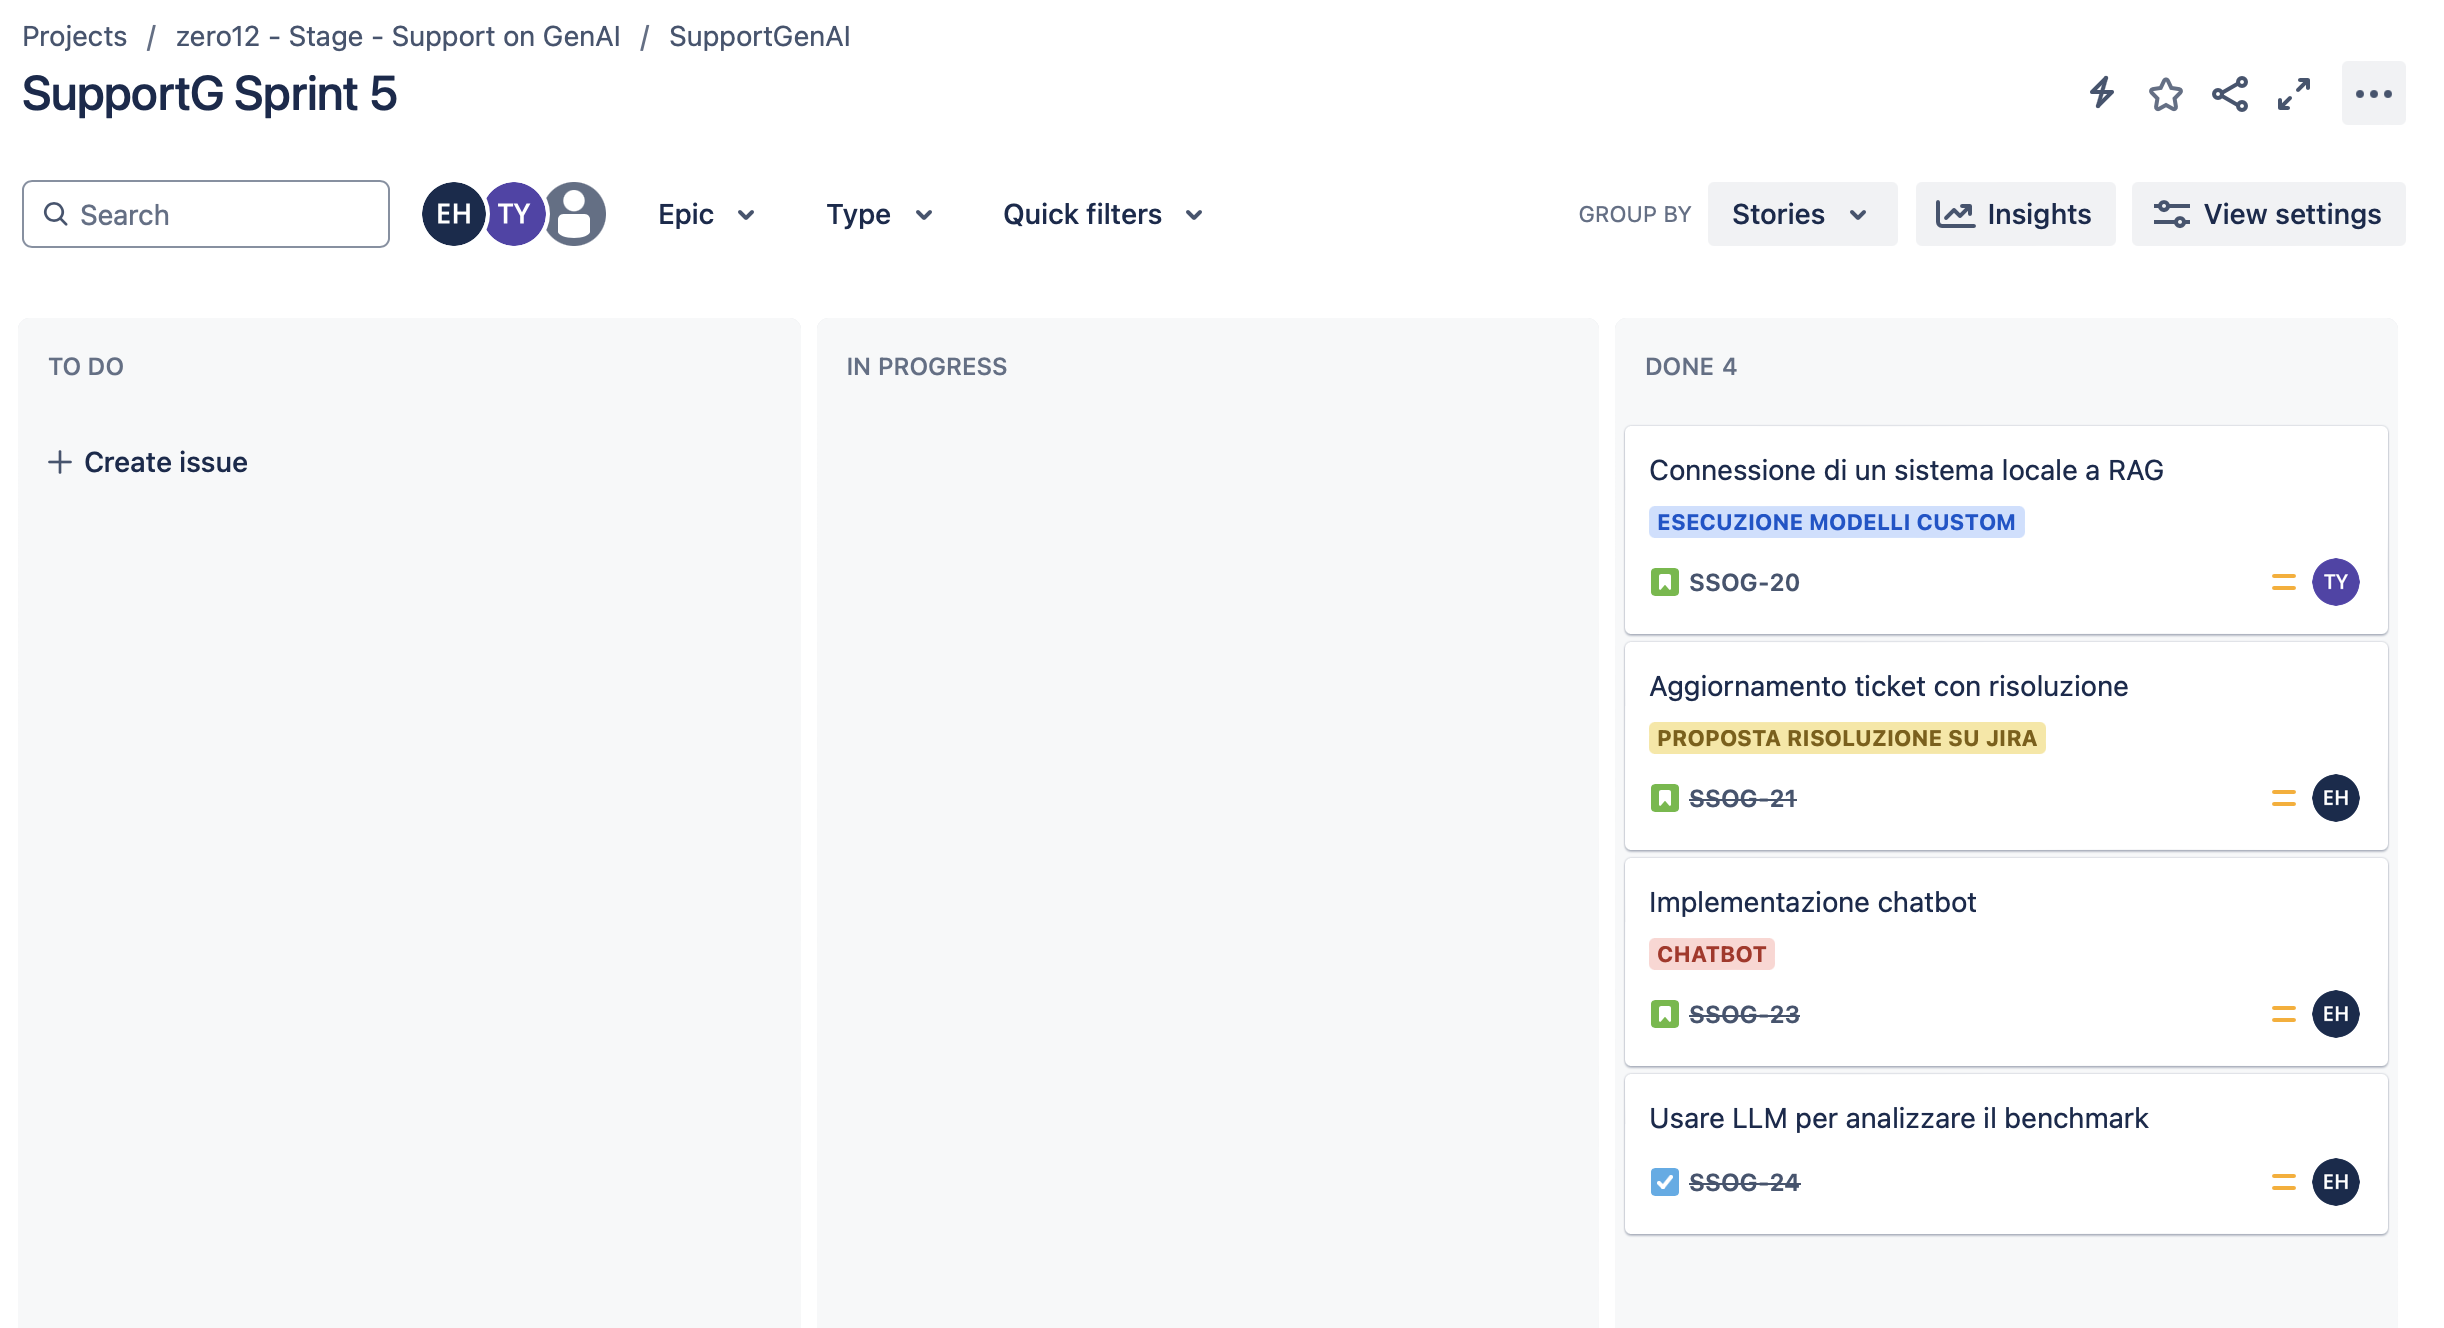
\includegraphics[width=0.7\textwidth]{Jira.png}
    \caption{\textit{Board} del quinto \textit{sprint} del progetto di \textit{stage}}
    \label{fig:Jira}
\end{figure}
\subsubsection{Visual Studio Code}
Visual Studio Code è un \textit{editor} di codice sorgente che permette la scrittura di codice in diversi linguaggi di programmazione.
\begin{figure}[H]
    \centering
    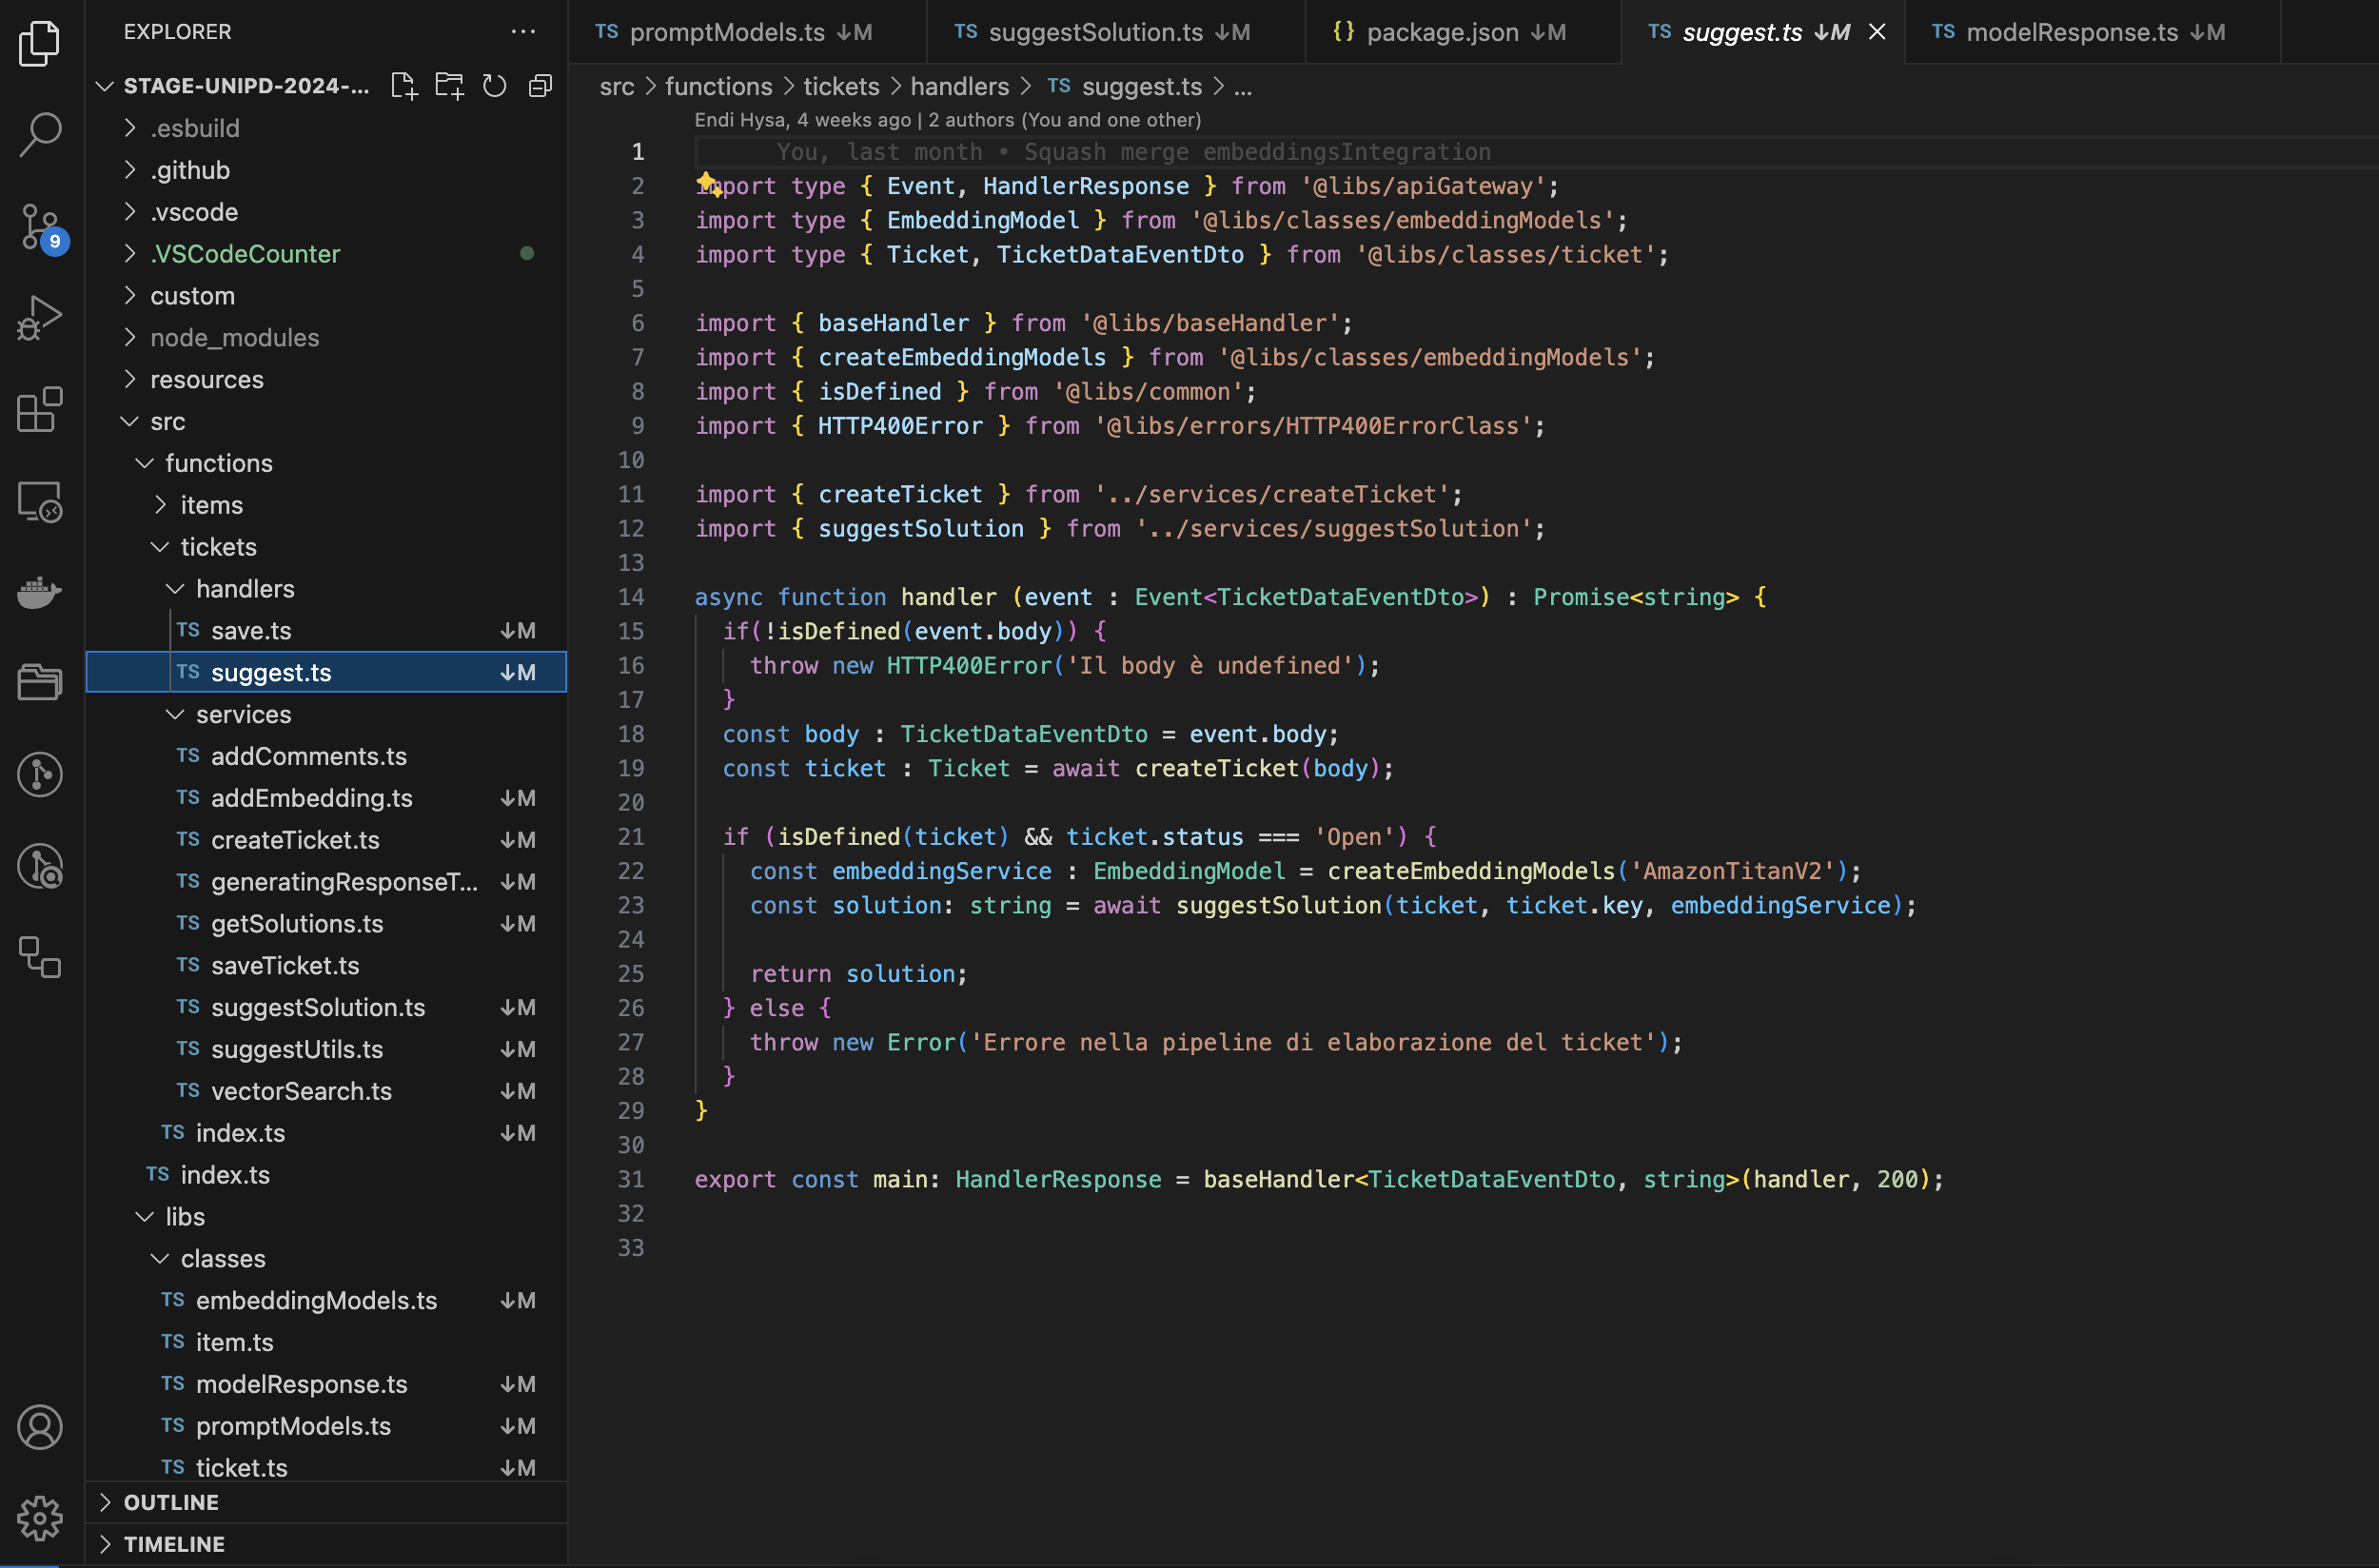
\includegraphics[width=0.7\textwidth]{VsCode.png}
    \caption{Schermata dell'\textit{editor} Visual Studio Code con codice Typescript}
    \label{fig:VsCode}
\end{figure}
\subsubsection{Github}
Github è una piattaforma \textit{web} che permette di usufruire del sistema di versionamento Git del codice sorgente, da interfaccia \textit{web}.
Grazie a questa piattaforma , è possibile creare \textit{repositories} in cui salvare il codice sorgente del progetto. 
È possibile suddividere il progetto in \textit{branch}, assegnati a specifiche \textit{feature} da sviluppare, permettendo cosi di lavorare in modo parallelo.
Terminata la codifica di una \textit{feature}, tramite una \textit{pull request}, si unisce il codice sviluppato nel \textit{branch} al codice sorgente presente nel \textit{branch} principale. Tramite \textit{pull request} il codice viene revisionato per garantire la sua qualità e la corretta integrazione con il codice sorgente principale.
\begin{figure}[H]
    \centering
    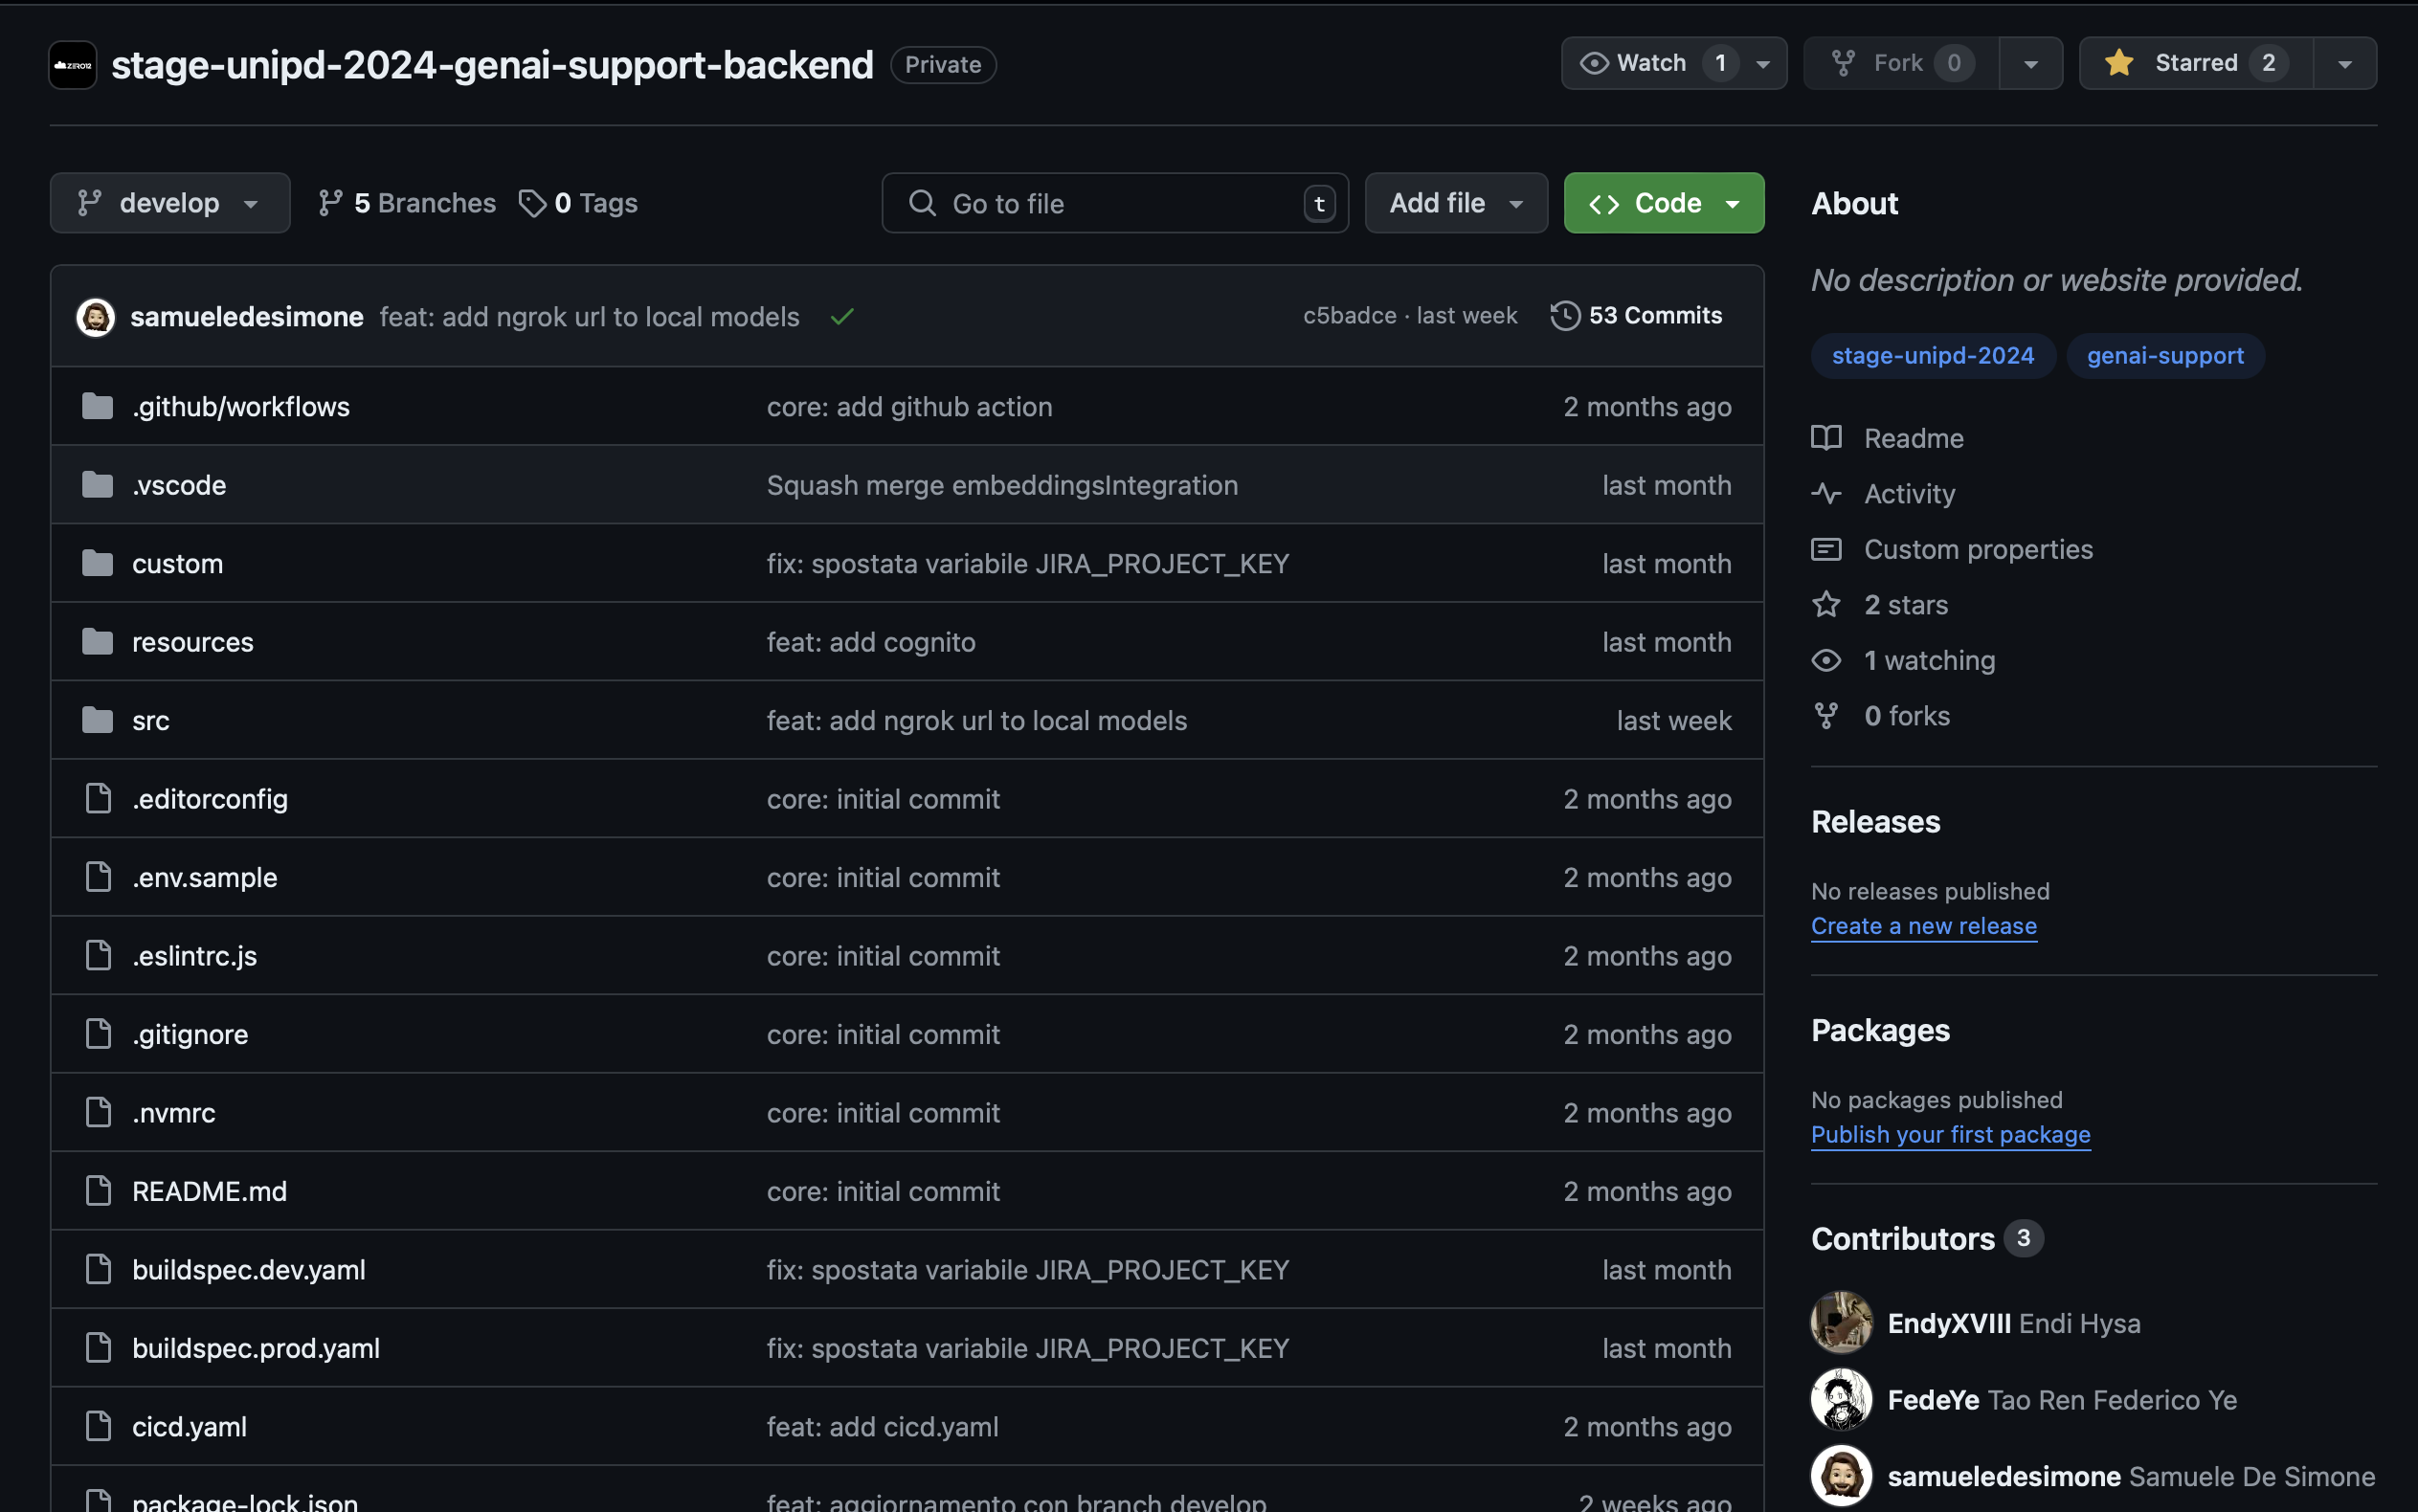
\includegraphics[width=0.7\textwidth]{github.png}
    \caption{Schermata del \textit{repository} Github del progetto di \textit{stage}}
    \label{fig:Github}
\end{figure}
\subsubsection{Slack}
Slack è un'applicazione di messaggistica utilizzata in ambito aziendale.
Permette la creazione di canali di comunicazione dedicati a specifici argomenti. Nel contesto aziendale, viene creato un canale dedicato ad ogni progetto in modo da poter permettere una comunicazione più efficace tra i membri del \textit{team} di lavoro.
Nel caso del mio progetto di \textit{stage}, è stato creato un canale dedicato al progetto assieme al mio \textit{tutor} aziendale ed un altra figura all'interno dell'azienda, con lo scopo aiutarmi in caso di problematiche durante la configurazione di alcuni servizi o durante lo sviluppo.
\begin{figure}[H]
    \centering
    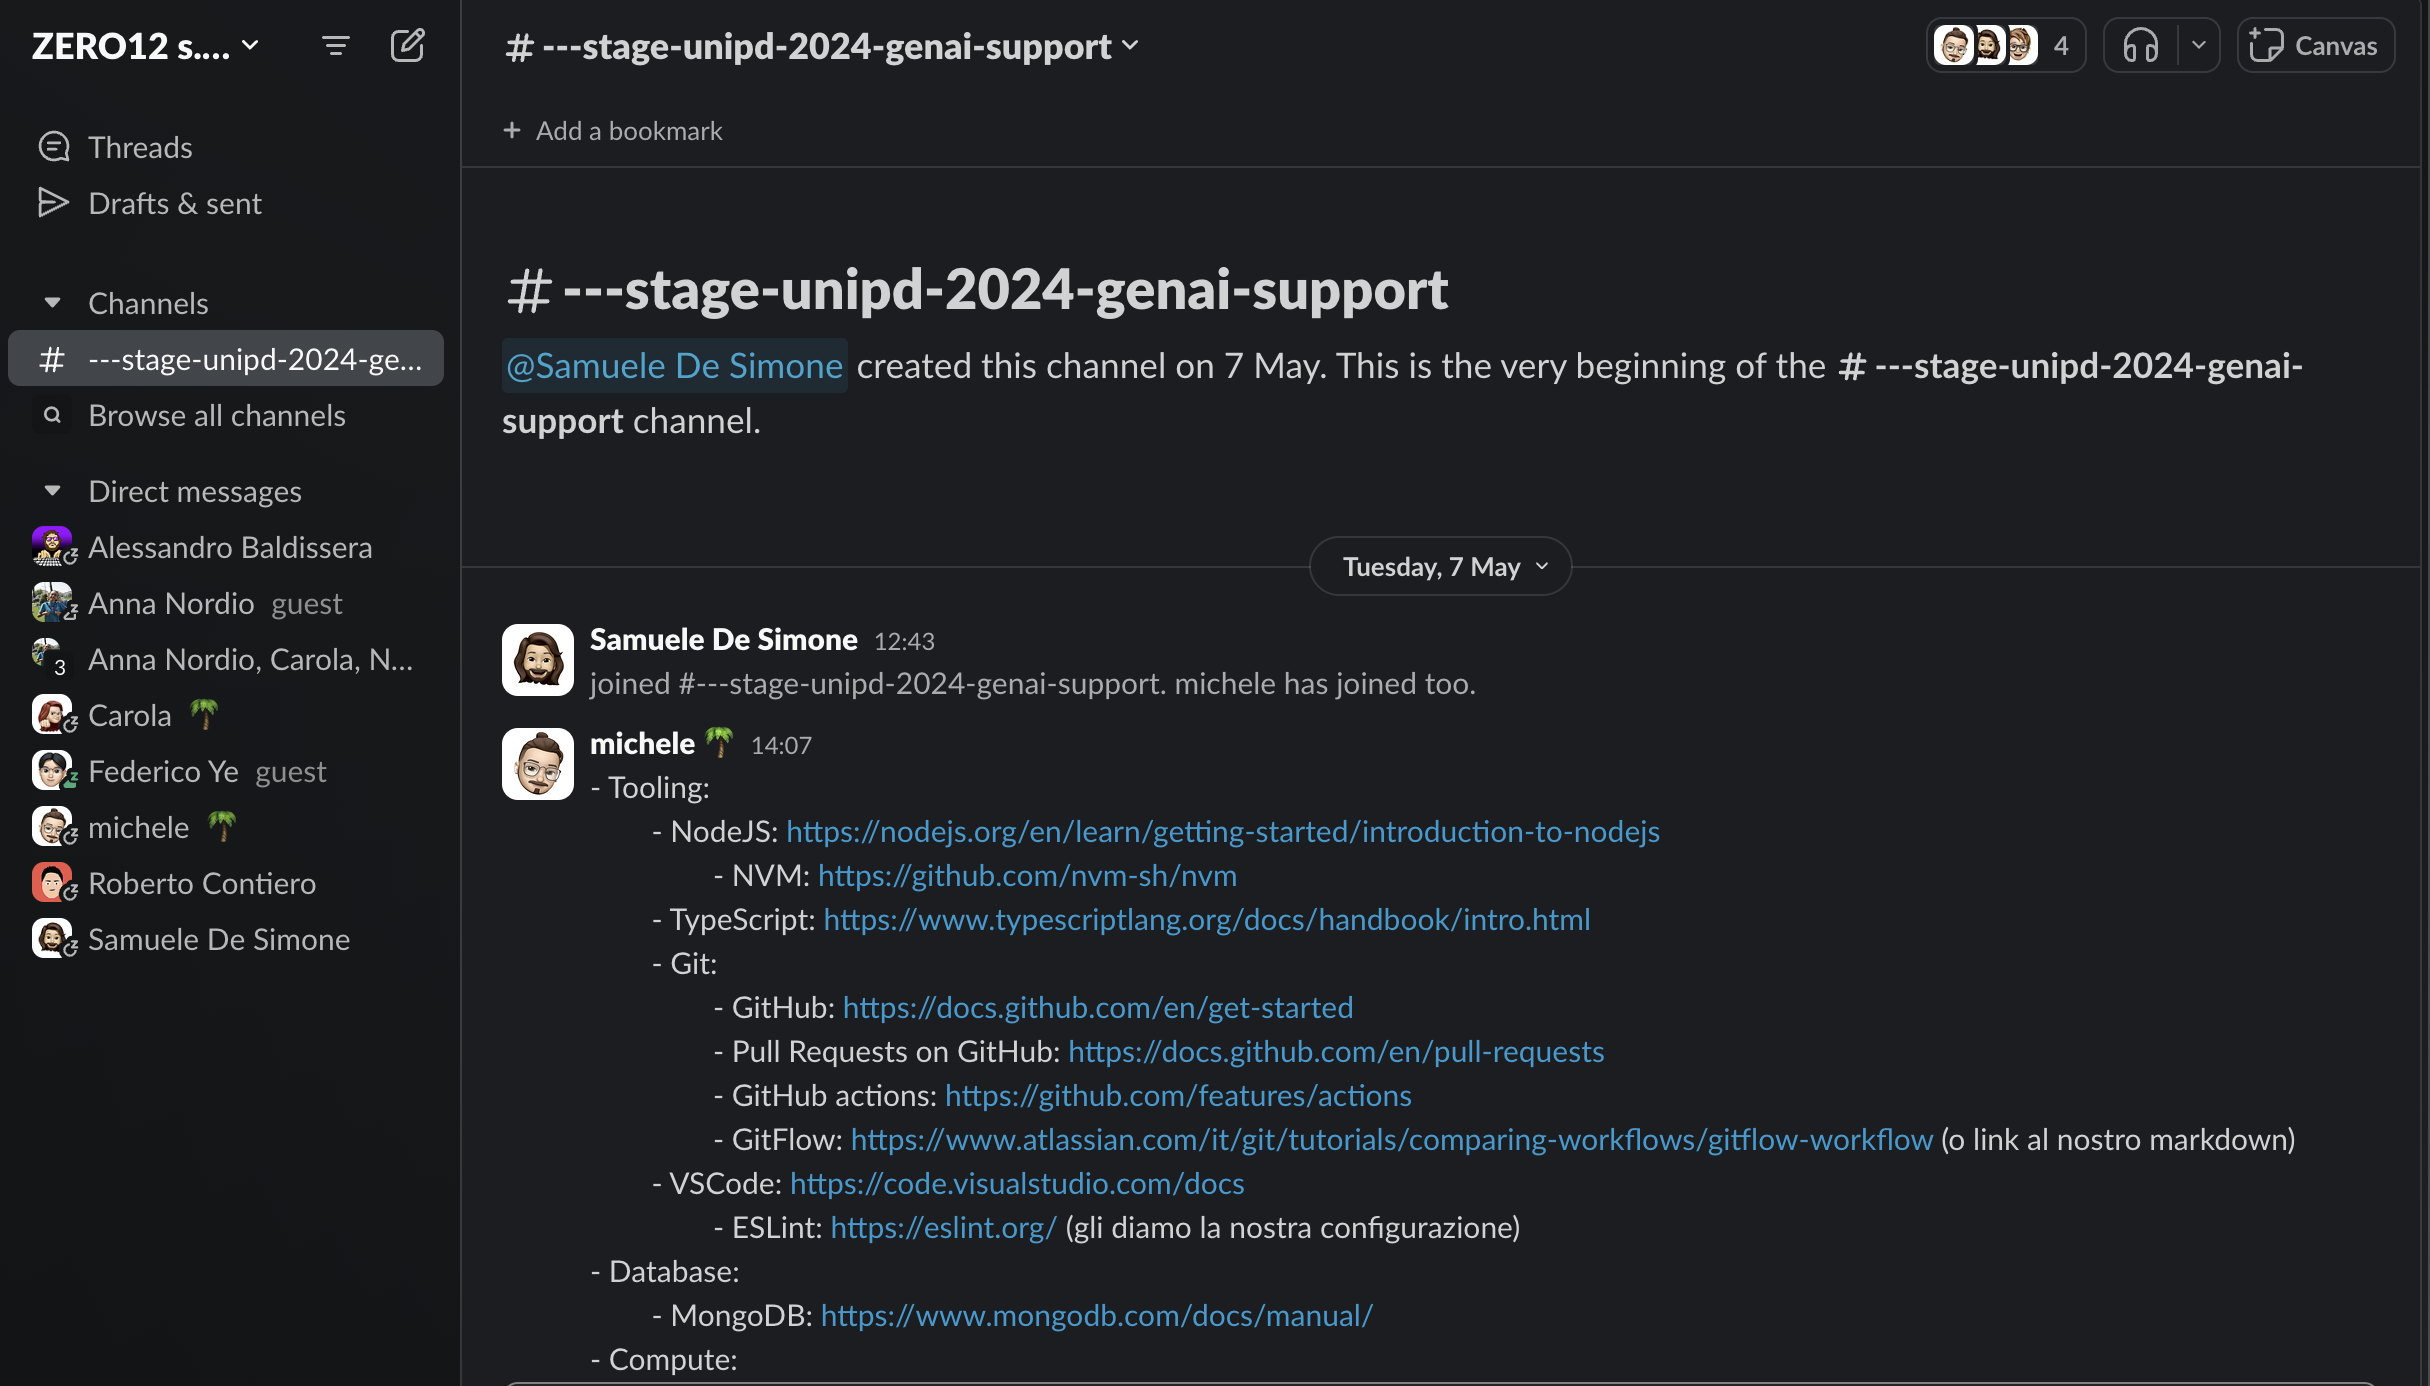
\includegraphics[width=0.66\textwidth]{slack.png}
    \caption{Schermata del canale dedicato al progetto di \textit{stage}}
    \label{fig:Slack}
\end{figure}
\noindent
Di seguito uno schema riassuntivo in cui mostro l'interazione degli strumenti utilizzati durante il flusso di progetto.
\begin{figure}[H]
    \centering
    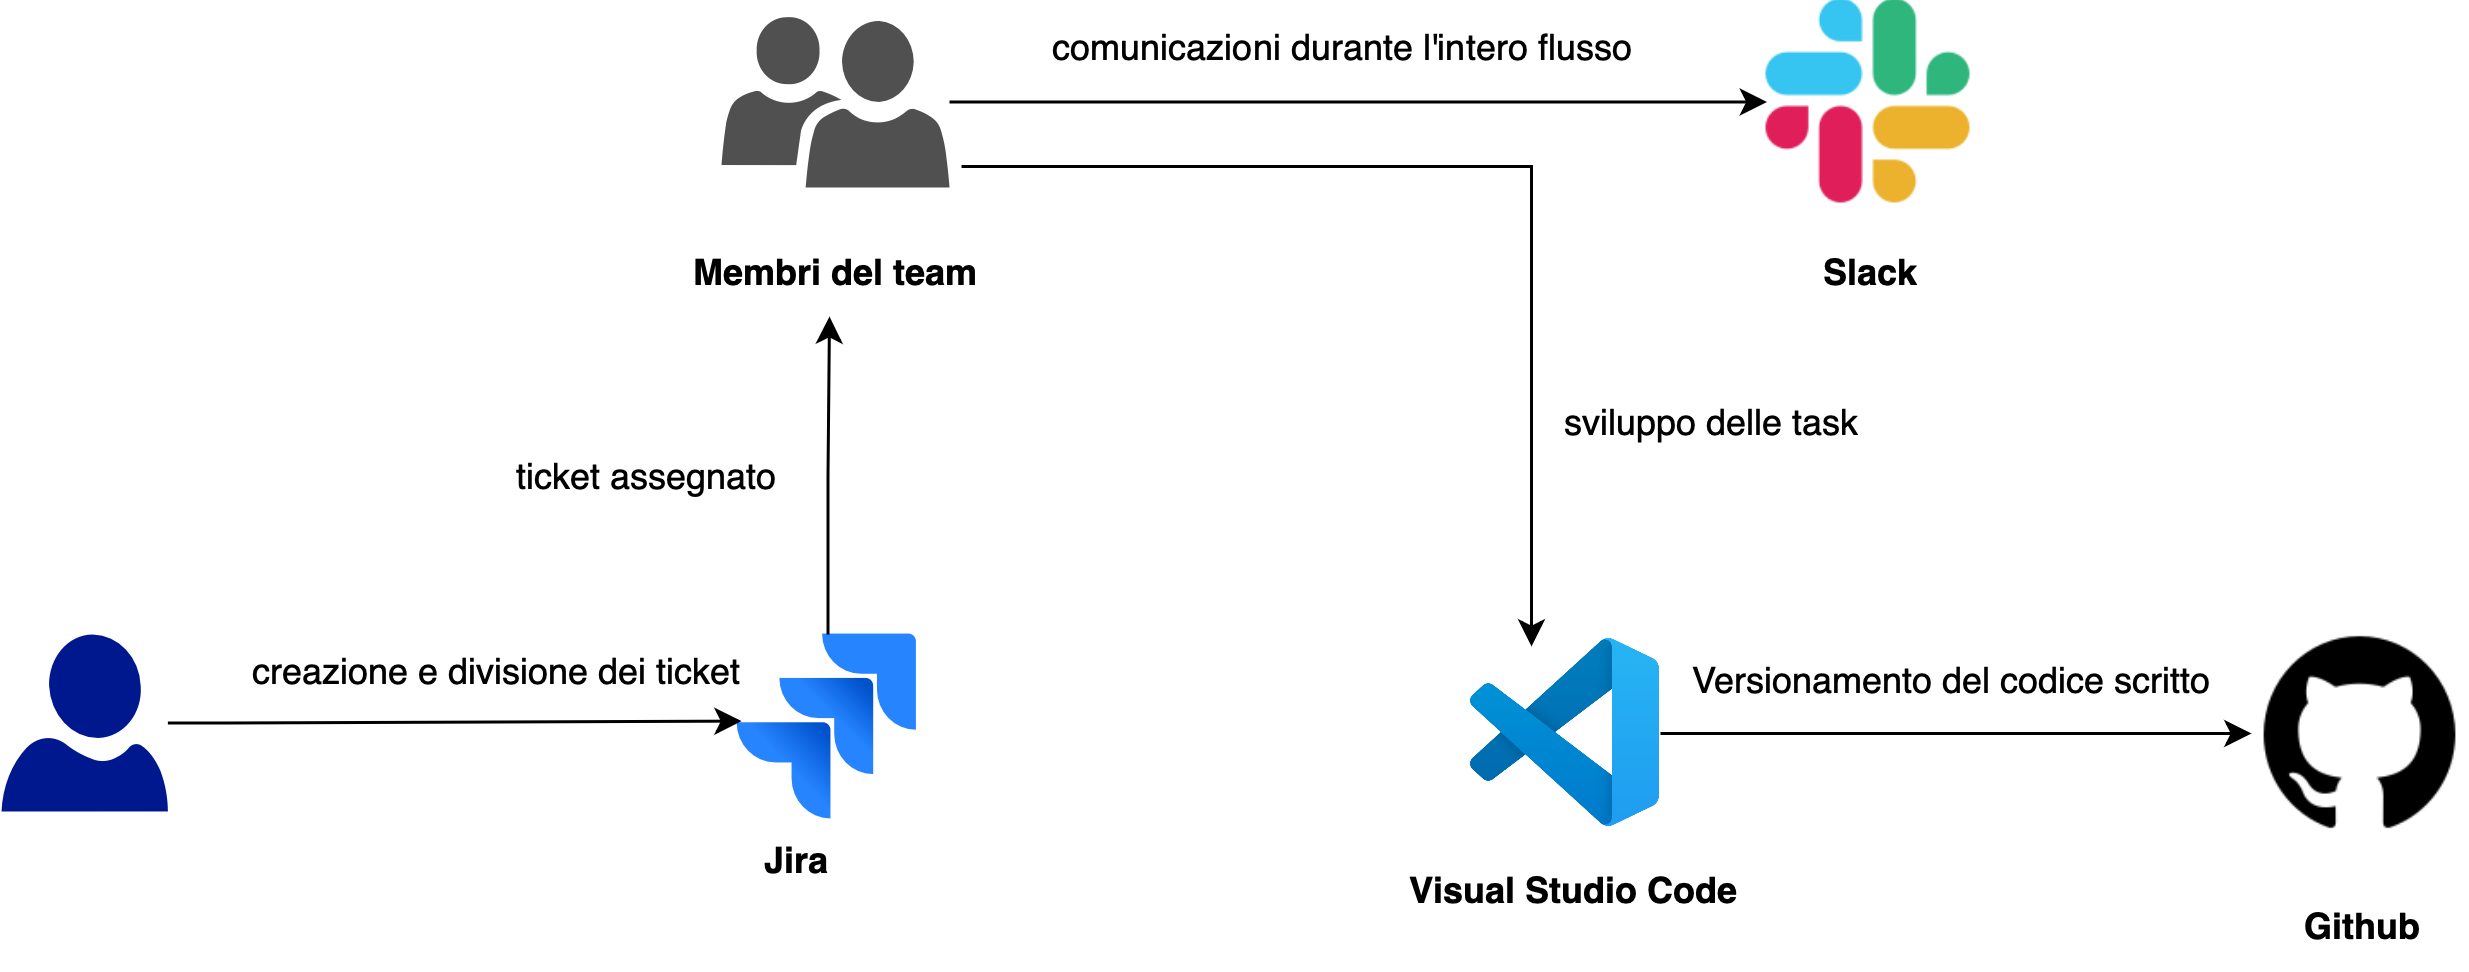
\includegraphics[width=0.88\textwidth]{sviluppoIntegrazione.png}
    \caption{Interazione degli strumenti nel processo di sviluppo}
    \small \textbf{Fonte:} \href{https://commons.wikimedia.org/wiki/File:Visual_Studio_Code_1.35_icon.svg}{Visual Studio: https://commons.wikimedia.org}

    \label{fig:sviluppoIntegrazione}
\end{figure}

\section{Tecnologie utilizzate} \label{sec:tecnologie}
\subsection{Tecnologie di sviluppo}
\subsubsection{Typescript}
TypeScript è un linguaggio di programmazione, noto per essere un \textit{superset} di JavaScript che introduce l'annotazione dei tipi. Essendo un \textit{superset} di JavaScript, ogni programma scritto in Javascript può essere eseguito anche in Typescript.
\begin{figure}[H]
    \centering
    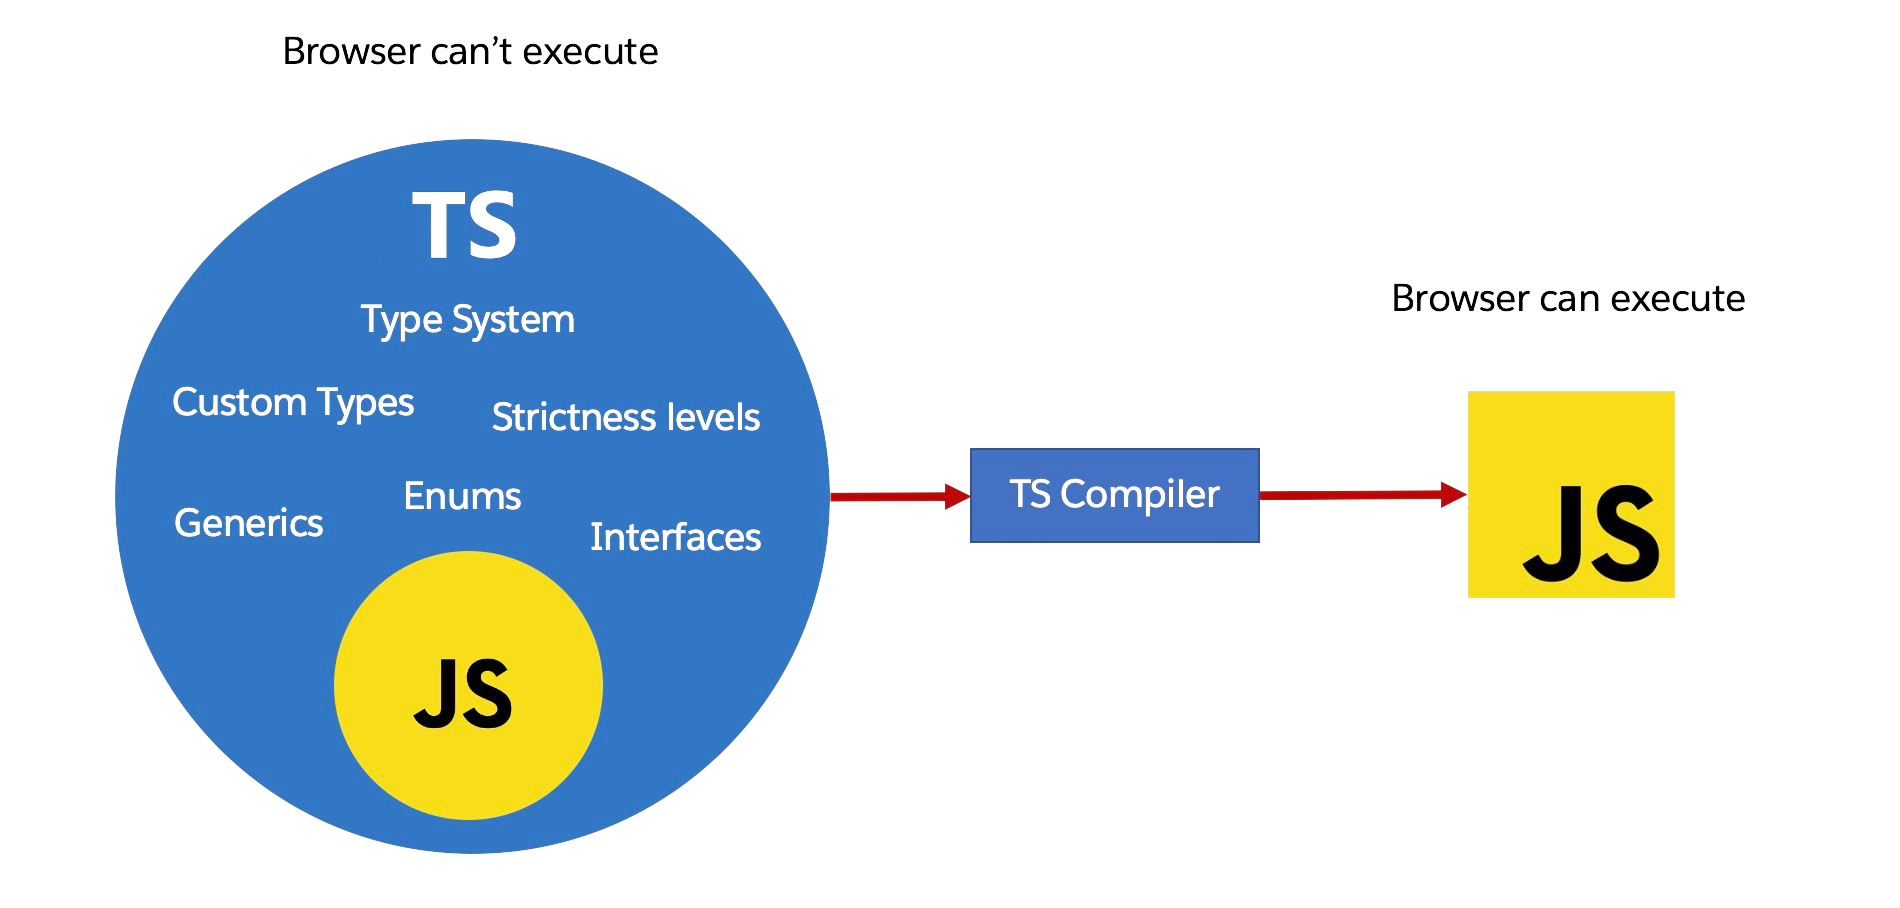
\includegraphics[width=0.7\textwidth]{typescriptjs.png}
    \caption{Funzionalità aggiuntive di Typescript rispetto a Javascript}
    \label{fig:Typescript}
\end{figure}
\subsubsection{Python}
Python è linguaggio di programmazione interpretato, ad alto livello. È orientato agli oggetti ed è adatto a molteplici utilizzi. Offre numerose librerie che permettono lo sviluppo di varie tipologie di applicazioni. 
\subsubsection{Node.js}
Node.js è un ambiente \textit{runtime} che consente di eseguire codice Javascript e Typescript al di fuori di un \textit{browser}. È basato sul motore JavaScript V8 e offre una libreria \textit{standard} che comprende vari moduli per le operazioni di base. 
\subsubsection{MongoDB}
MongoDB è un \textit{database} non relazionale (\textit{NoSQL}) dove i dati non vengono strutturati in tabelle con uno schema preciso, ma vengono raggruppati in documenti dove la struttura dei dati può variare da documento a documento. Permette di salvare oltre ai dati anche i loro relativi \gls{embedding-g}, ovvero una rappresentazione numerica vettoriale dell'oggetto in uno spazio multidimensionale.
\begin{figure}[H]
    \centering
    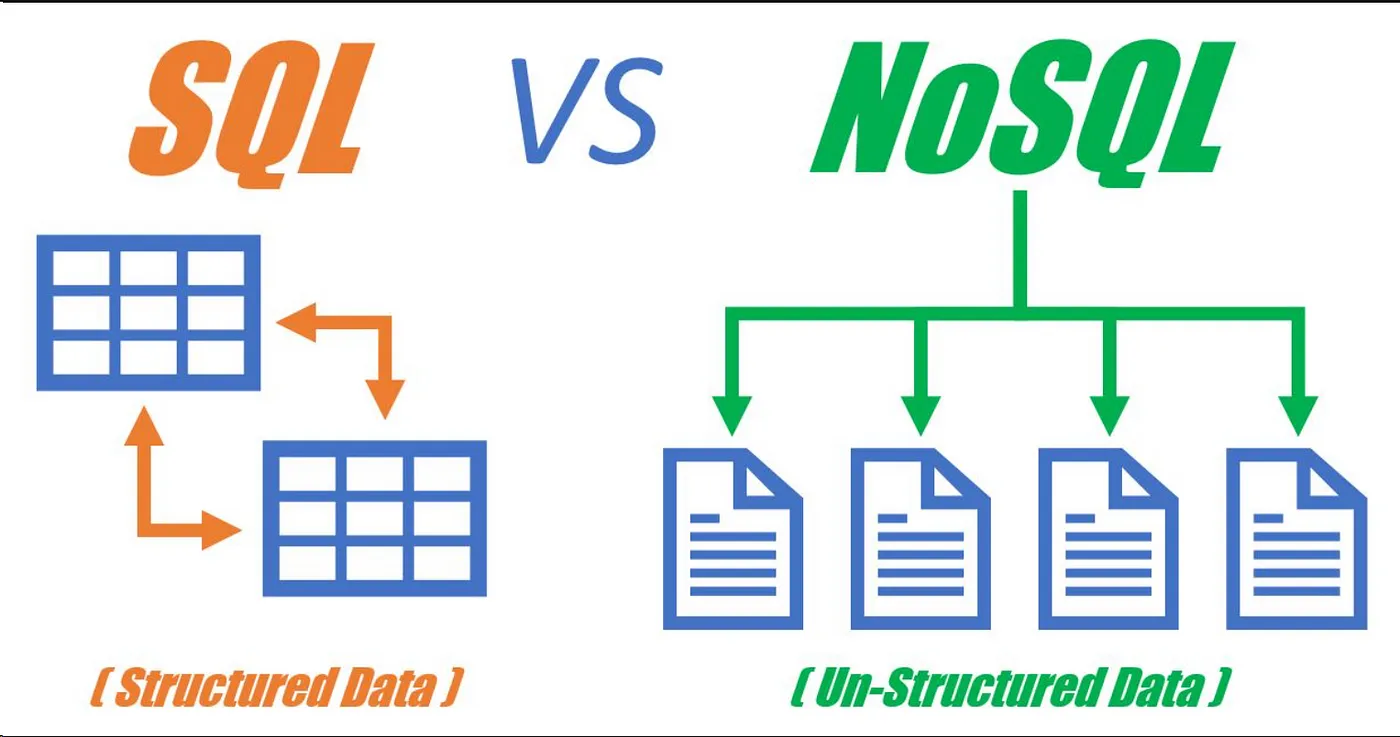
\includegraphics[width=0.48\textwidth]{sqlvsnosql.png}
    \caption{Differenza tra la struttura di un \textit{database} relazionale e un \textit{database} non relazionale}
    \small \textbf{Fonte:} \href{https://naveen-metta.medium.com/decoding-the-database-dilemma-sql-vs-nosql-in-system-design-8666e21f4a58c}{medium.com}
    \label{fig:sql-vs-nosql}
\end{figure} 

\subsubsection{Serverless framework}
Il Serverless \textit{framework} è un \textit{framework} che permette la creazione di \gls{api}, un' interfaccia che definisce come due parti (applicazione \textit{client} e \textit{server}) comunicano tra loro usando richieste e risposte, su infrastuttura \gls{aws}. Permette la definizione di funzioni \textit{lambda} con i relativi \textit{trigger} di invocazione e il \textit{deploy} nel \textit{cloud}, attraverso un semplice comando che carica il codice sorgente e configura l'architettura in modo automatico. Supporta diversi \textit{plugin} che permettono l'utilizzo di altri servizi offerti da \gls{aws}.
\begin{figure}[H]
    \centering
    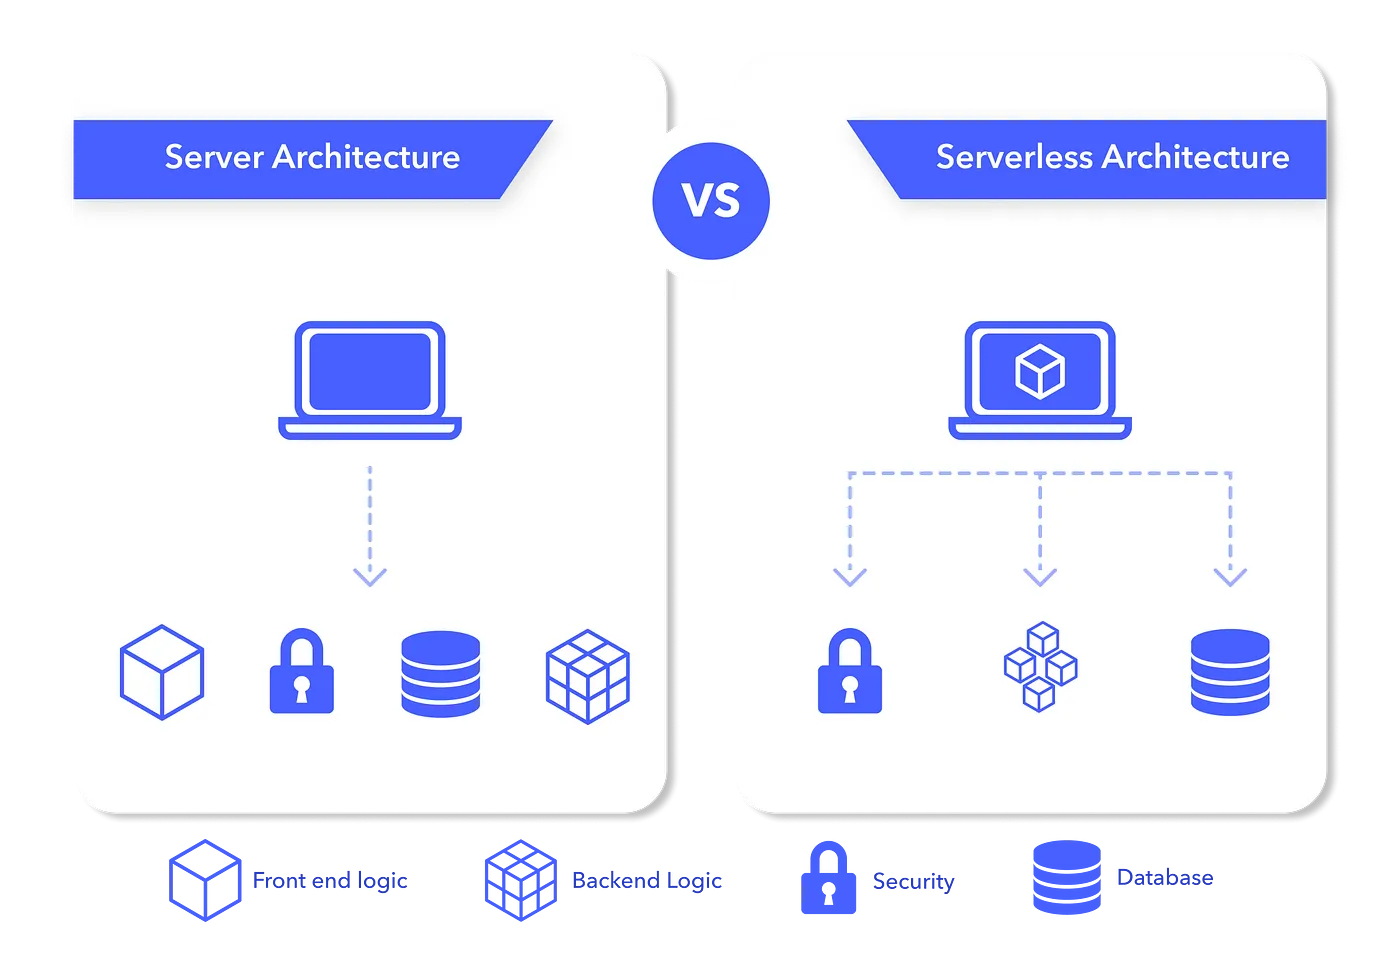
\includegraphics[width=0.68\textwidth]{serverless.png}
    \caption{Confronto tra un'architettura tradizionale e un' architettura \textit{\gls{serverlessg}}}
    \small \textbf{Fonte:} \href{https://medium.com/canonichq/server-v-s-serverless-architecture-bf3cdab28174}{medium.com}
    \label{fig:Serverless}
\end{figure} 
\noindent
Come mostro nella figura \ref{fig:Serverless}, l'architettura \textit{\gls{serverlessg}} permette all'utente di non doversi preoccupare della gestione dell'infrastruttura sottostante, in quanto viene gestita automaticamente dal fornitore del servizio. Nella controparte dell'architettura tradizionale, l'utente deve gestire l'infrastruttura sottostante.
\subsubsection{Streamlit}
Streamlit è un \textit{framework open-source} che permette la creazione di applicazioni \textit{web} per la visualizzazione di dati in modo rapido e semplice.
Con il suo utilizzo, si possono trasformare \textit{script} Python in applicazioni \textit{web} interattive.
\begin{figure}[H]
    \centering
    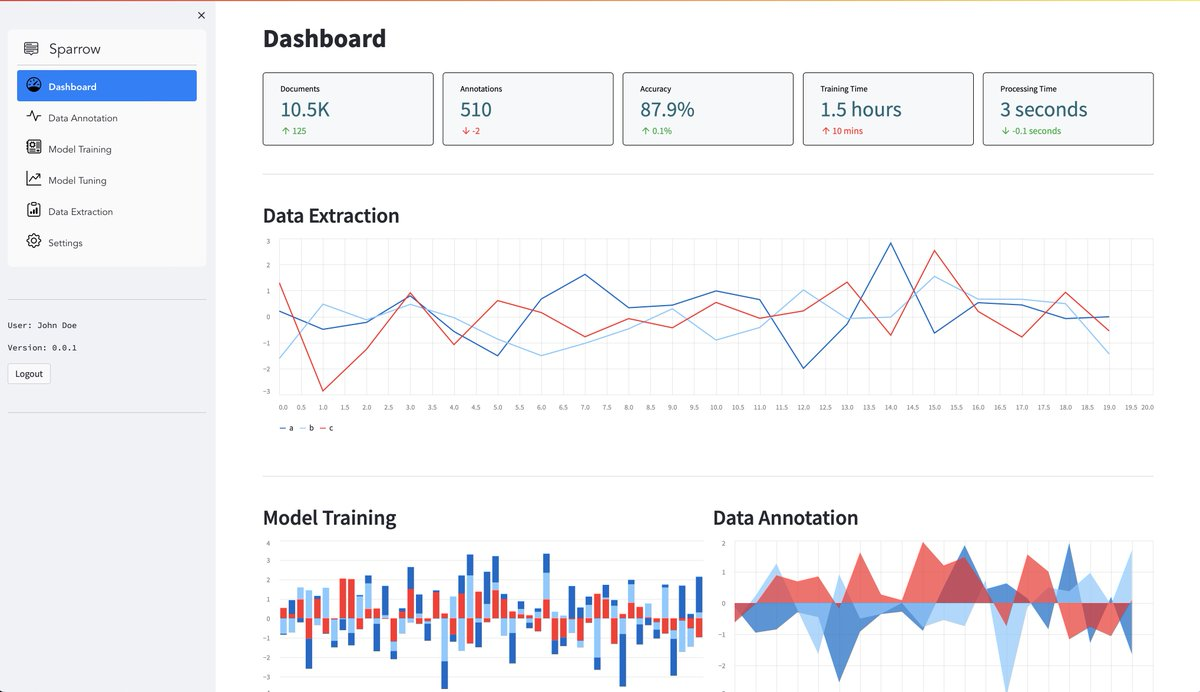
\includegraphics[width=0.7\textwidth]{streamlit.png}
    \caption{Esempio di applicazione \textit{web} creata con il \textit{framework} Streamlit}
    \small \textbf{Fonte:} \href{https://streamlit.io}{streamlit.io}
    \label{fig:Streamlit}
\end{figure} 

\subsubsection{LangChain}
Langchain è un \textit{framework open-source} che fornisce strumenti e componenti modulari per la creazione di applicazioni, come \textit{chatbot}, che sfruttano i \gls{llm}. Questo \textit{framework} permette un' interazione più semplice con questi modelli, permettendo di creare applicazioni che sfruttano le potenzialità dei \gls{llm} in modo più semplice. Nel contesto dello \textit{stage}, viene utilizzato assieme al \textit{framework} Streamlit.
\begin{figure}[H]
    \centering
    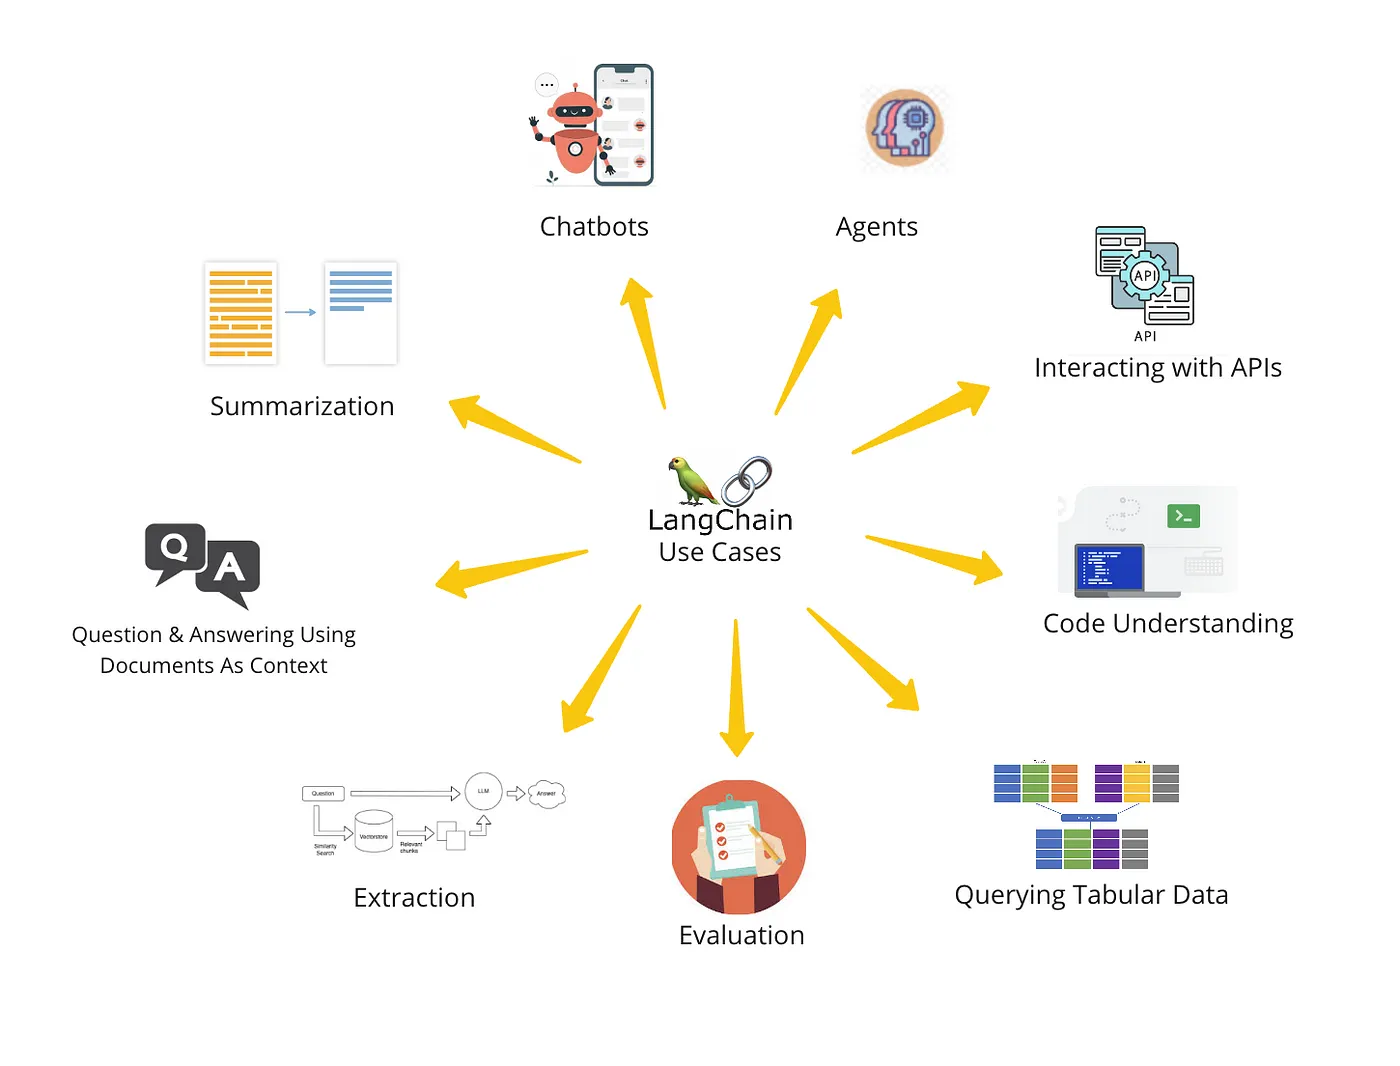
\includegraphics[width=0.73\textwidth]{langchain.png}
    \caption{Casi d'uso con Langchain} 
    \small \textbf{Fonte:} \href{https://medium.com/@ebruboyaci/use-cases-with-langchain-e0fd5b0587f1}{https://medium.com}
    \label{fig:Lanchain}
\end{figure} 

\subsubsection {Servizi AWS}
Nella realizzazione del progetto di \textit{stage} sono stati utilizzati diversi servizi offerti da \gls{aws}. I servizi principali utilizzati sono:
\begin{itemize}
    \item \textbf{AWS Lambda}: servizio che permette l'esecuzione di codice senza la necessità di dover gestire \textit{server} sottostanti. Sono autoscalabili in base al carico di lavoro. Generalmente sono funzioni che seguono il \textit{Simple Responsability Principle}.
    \item \textbf{AWS Bedrock}: servizio che permette l'utilizzo di vari modelli di \textit{machine learning} messi a disposizione, utilizzabili tramite chiamata \gls{api}.
    \item \textbf{AWS API Gateway}: servizio che permette la creazione, la pubblicazione, la manutenzione, il monitoraggio e la protezione di \gls{api} su larga scala. Si integra nell'ecosistema \gls{aws} offrendo \textit{trigger} di eventi per l'esecuzioni di funzioni \textit{lambda}.
    \item \textbf{AWS Cognito}: servizio che fornisce un sistema di autenticazione e autorizzazione per gli applicativi \textit{web} e \textit{mobile}. Gestisce automaticamente la registrazione di nuovi utenti, il \textit{login}, il recupero della \textit{password} e la gestione delle sessioni.
\end{itemize}
Alcuni servizi vengono utilizzati per attuare il processo di \gls{ci-cd}, una pratica di sviluppo in cui tutte le modifiche apportate al \textit{software} durante lo sviluppo, vengono integrate e testate automaticamente, garantendo che il codice sia sempre funzionante e pronto per il rilascio.
\subsection{Tecnologie per la validazione del codice}
\subsubsection{ESLint}
ESLint è un \textit{plugin} installato su Visual Studio Code che permette il controllo del codice in fase di scrittura, segnando eventuali errori di sintassi o di stile.
È possibile impostare una configurazione personalizzata (come l'indentazione del codice, la lunghezza delle righe, ecc.), permettendo così di scrivere codice uniforme agli \textit{standard} aziendali.
\begin{figure}[H]
    \centering
    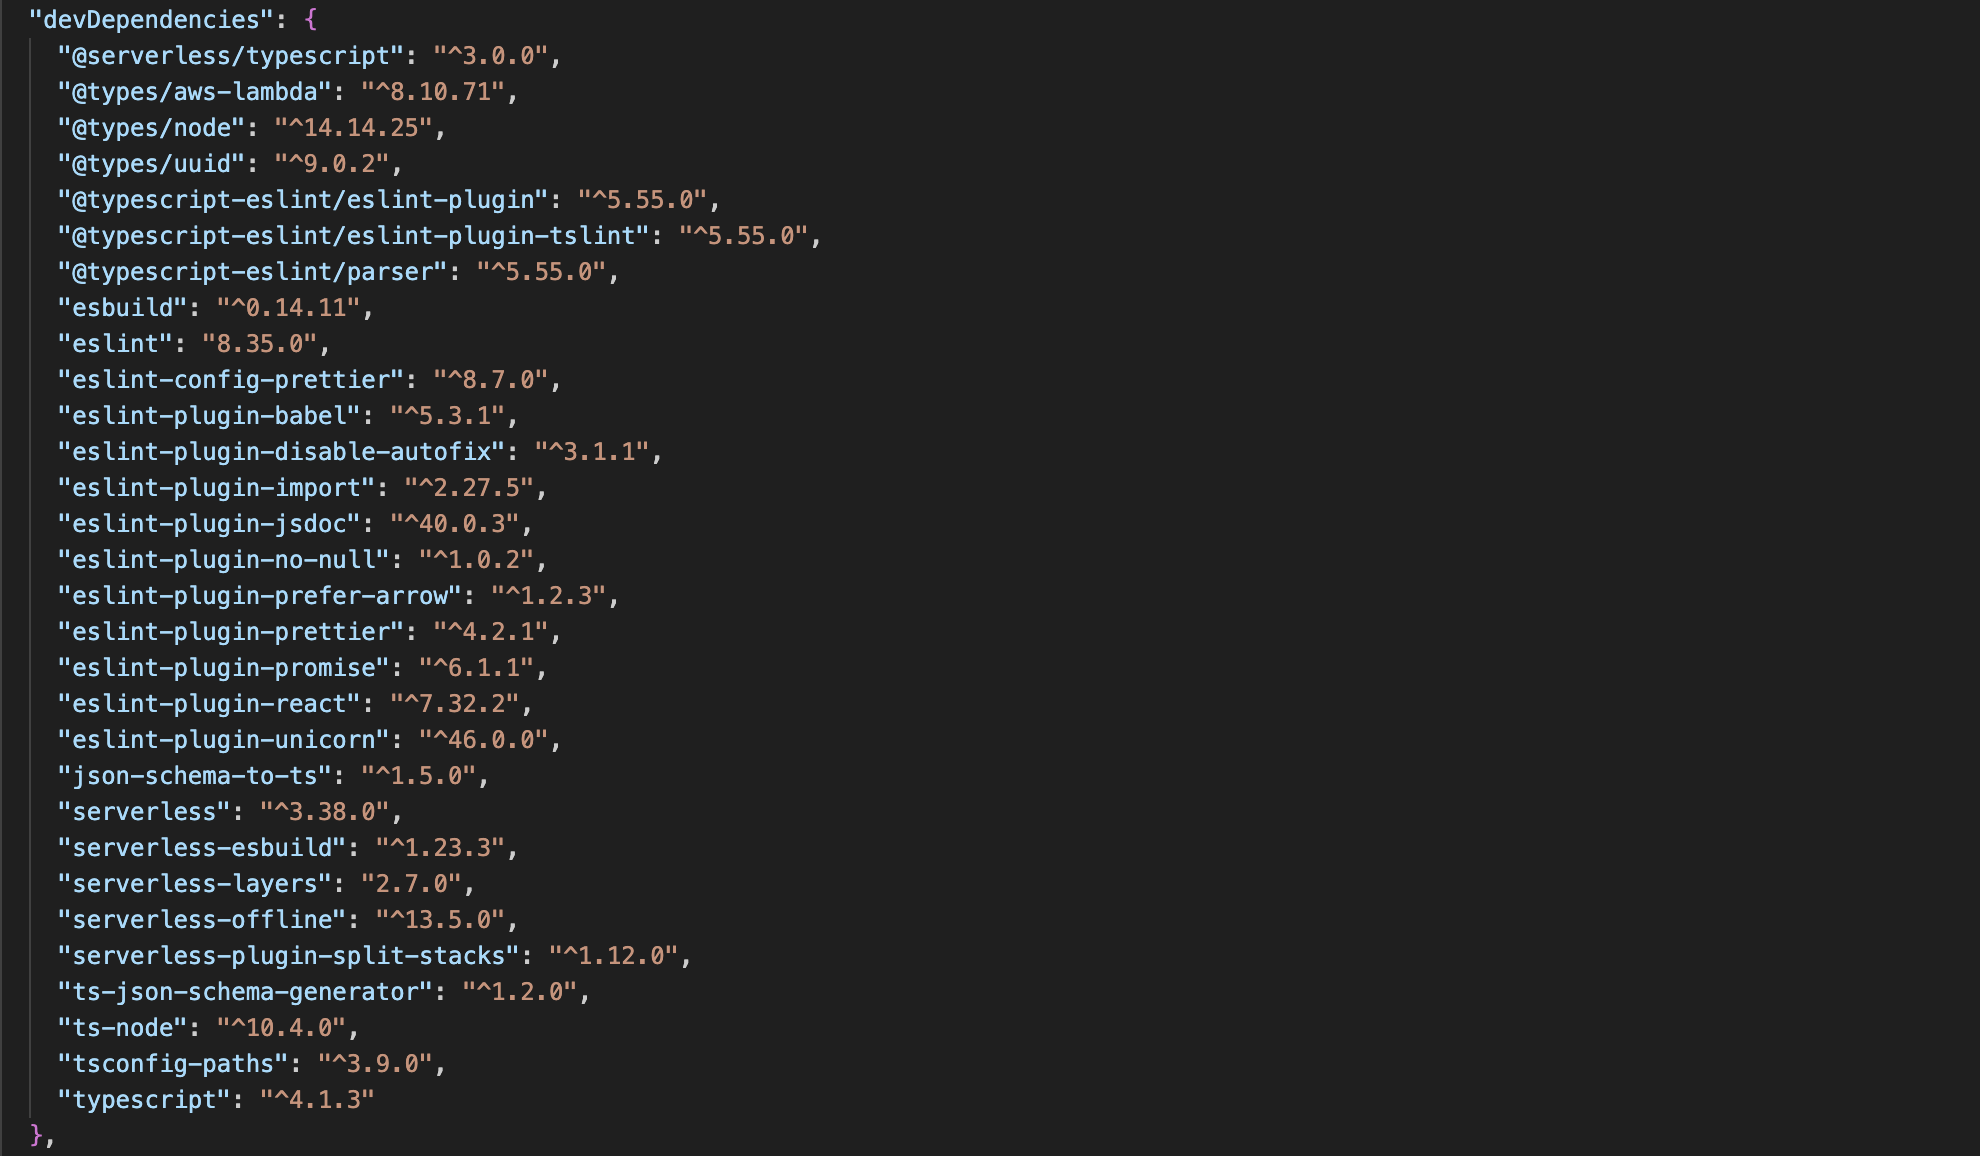
\includegraphics[width=0.83\textwidth]{eslint.png}
    \caption{Esempio di configurazione di ESLint}
    \label{fig:ESlint}
\end{figure} 
\subsection{Tecnologie di supporto}
\subsubsection{Postman}
Postman è un \textit{software} che permette il salvataggio e il testing di \gls{api} in modo semplice. Tramite l'interfaccia è possibile organizzare le richieste e generare documentazione delle \gls{api} salvate.
\begin{figure}[H]
    \centering
    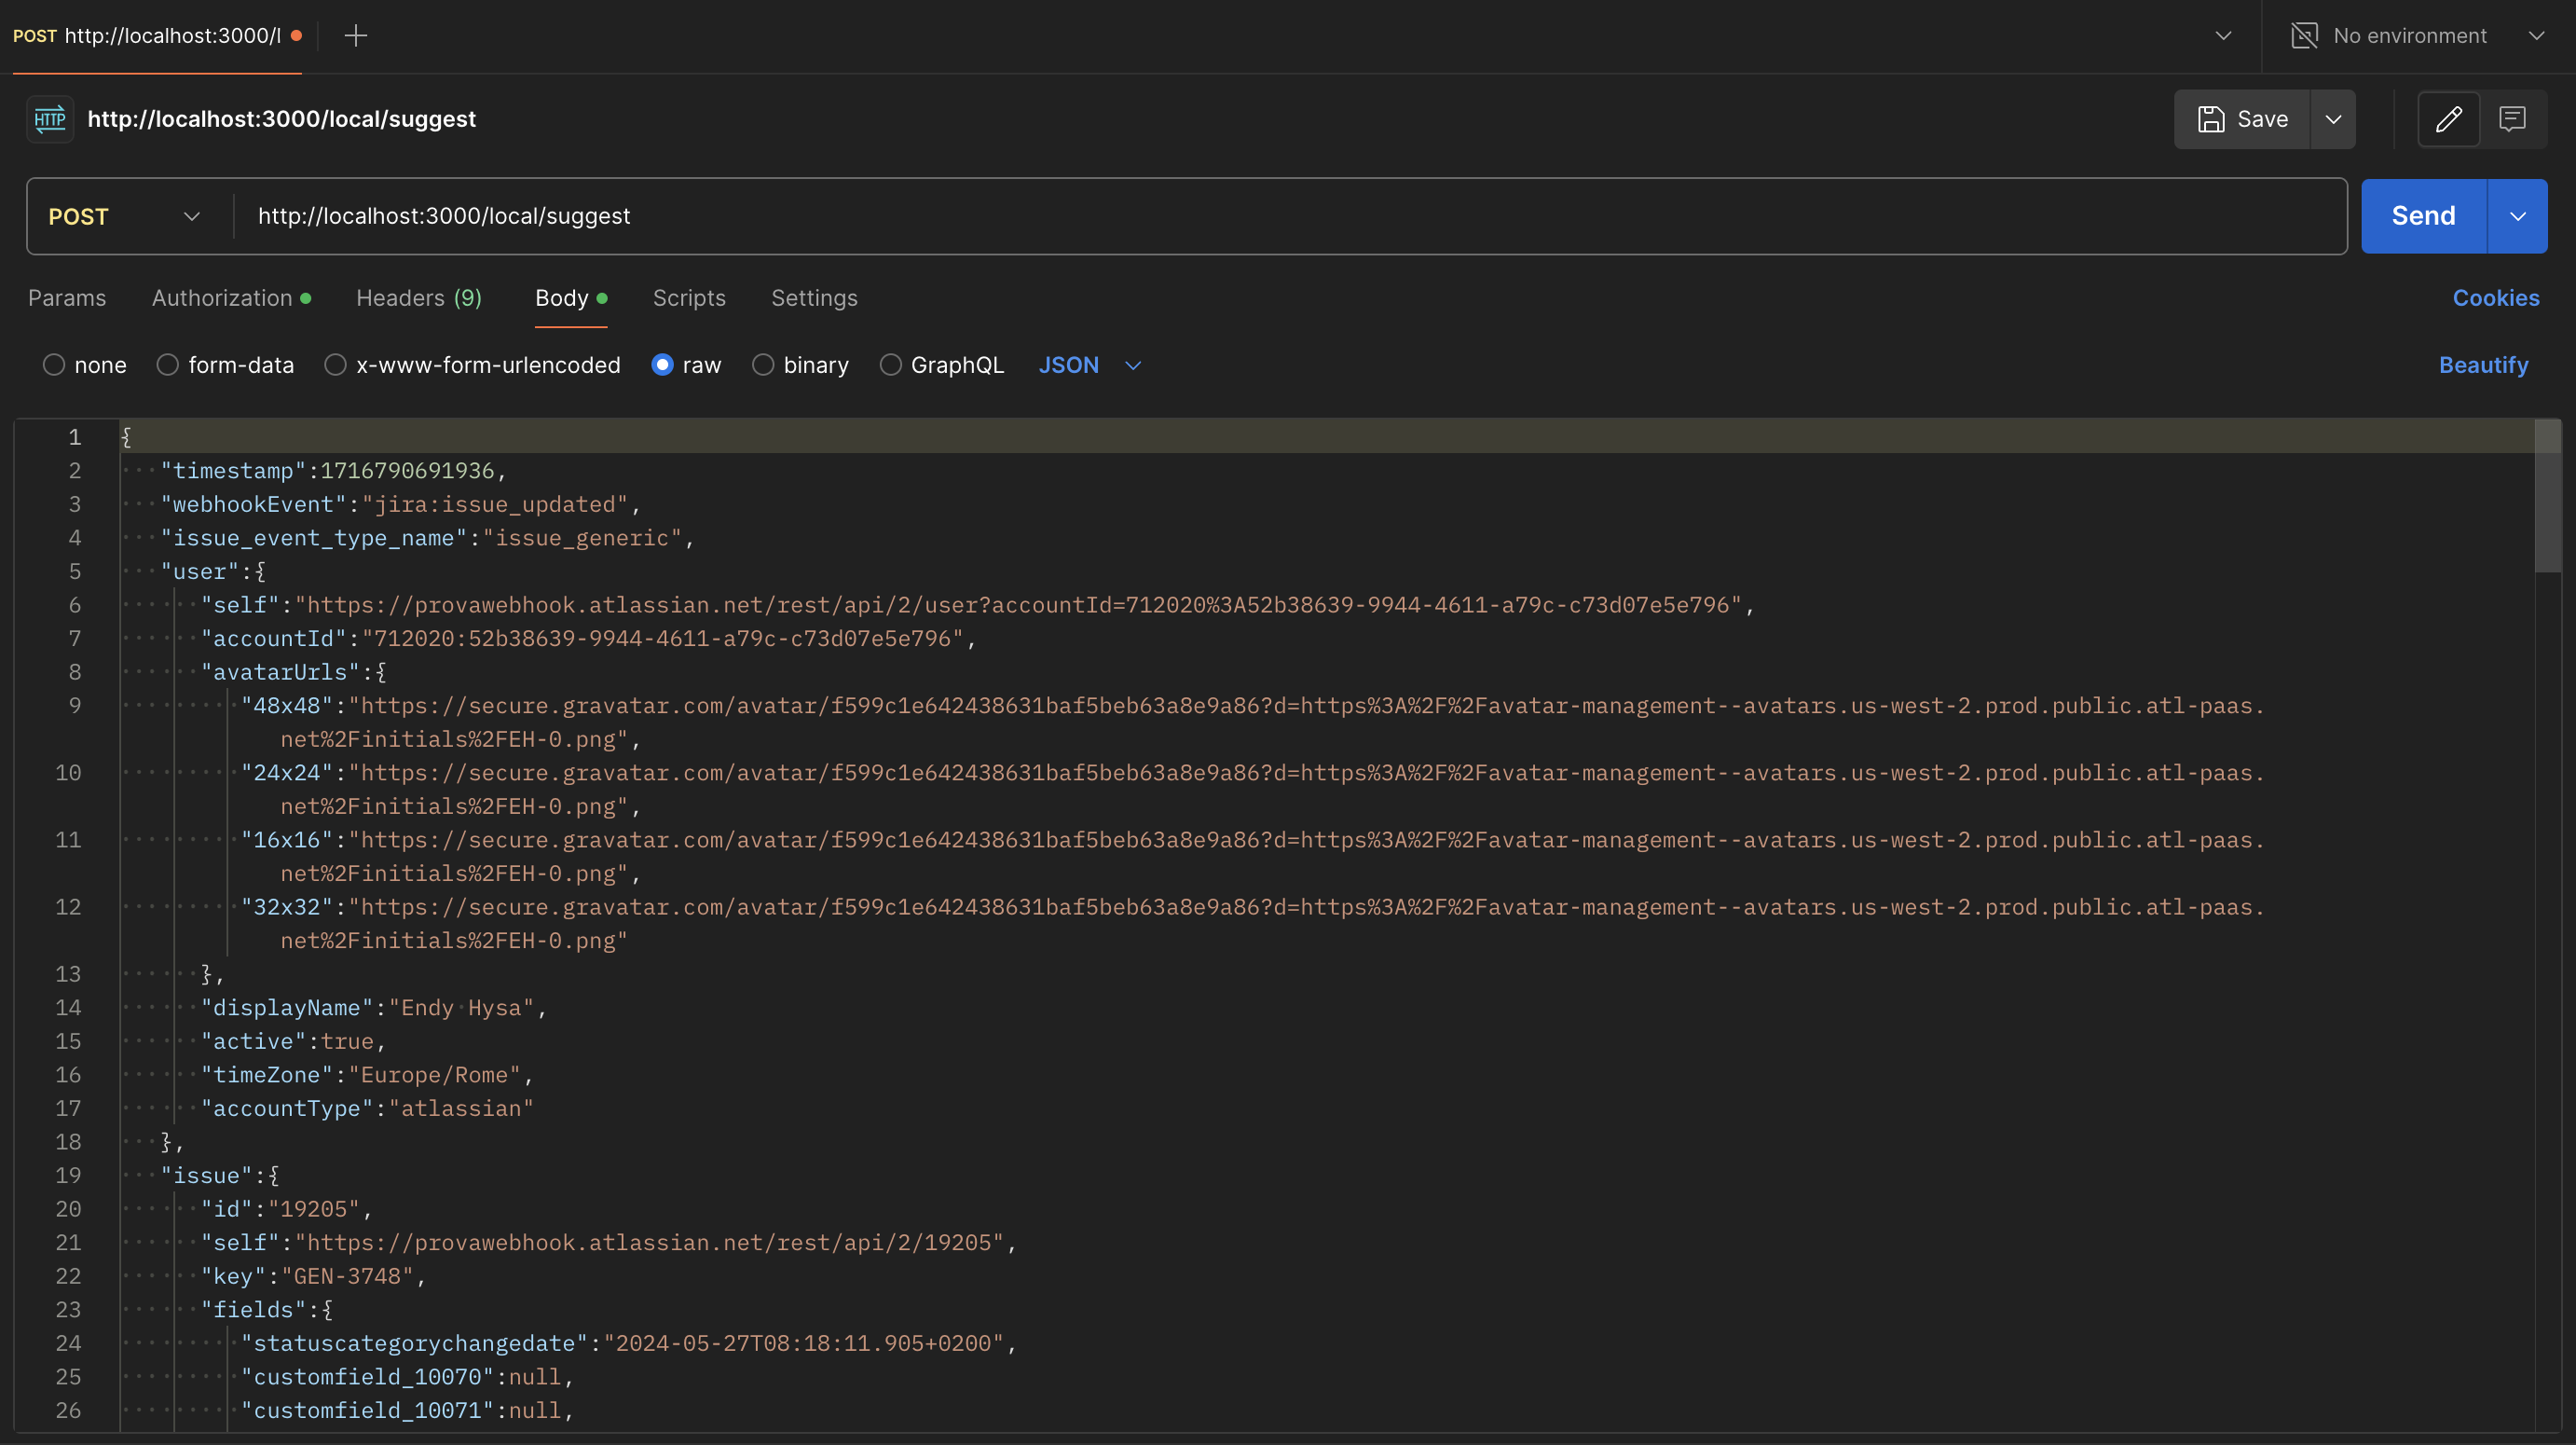
\includegraphics[width=0.85\textwidth]{postman.png}
    \caption{Esempio di API di tipo \textit{POST} su Postman con relativo \textit{body}}
    \label{fig:Postman}
\end{figure} 



\subsubsection{MongoDB Compass}
MongoDB Compass è un \textit{software} che permette la visualizzazione dei documenti salvati nel \textit{database} MongoDB tramite un'interfaccia grafica.
\begin{figure}[H]
    \centering
    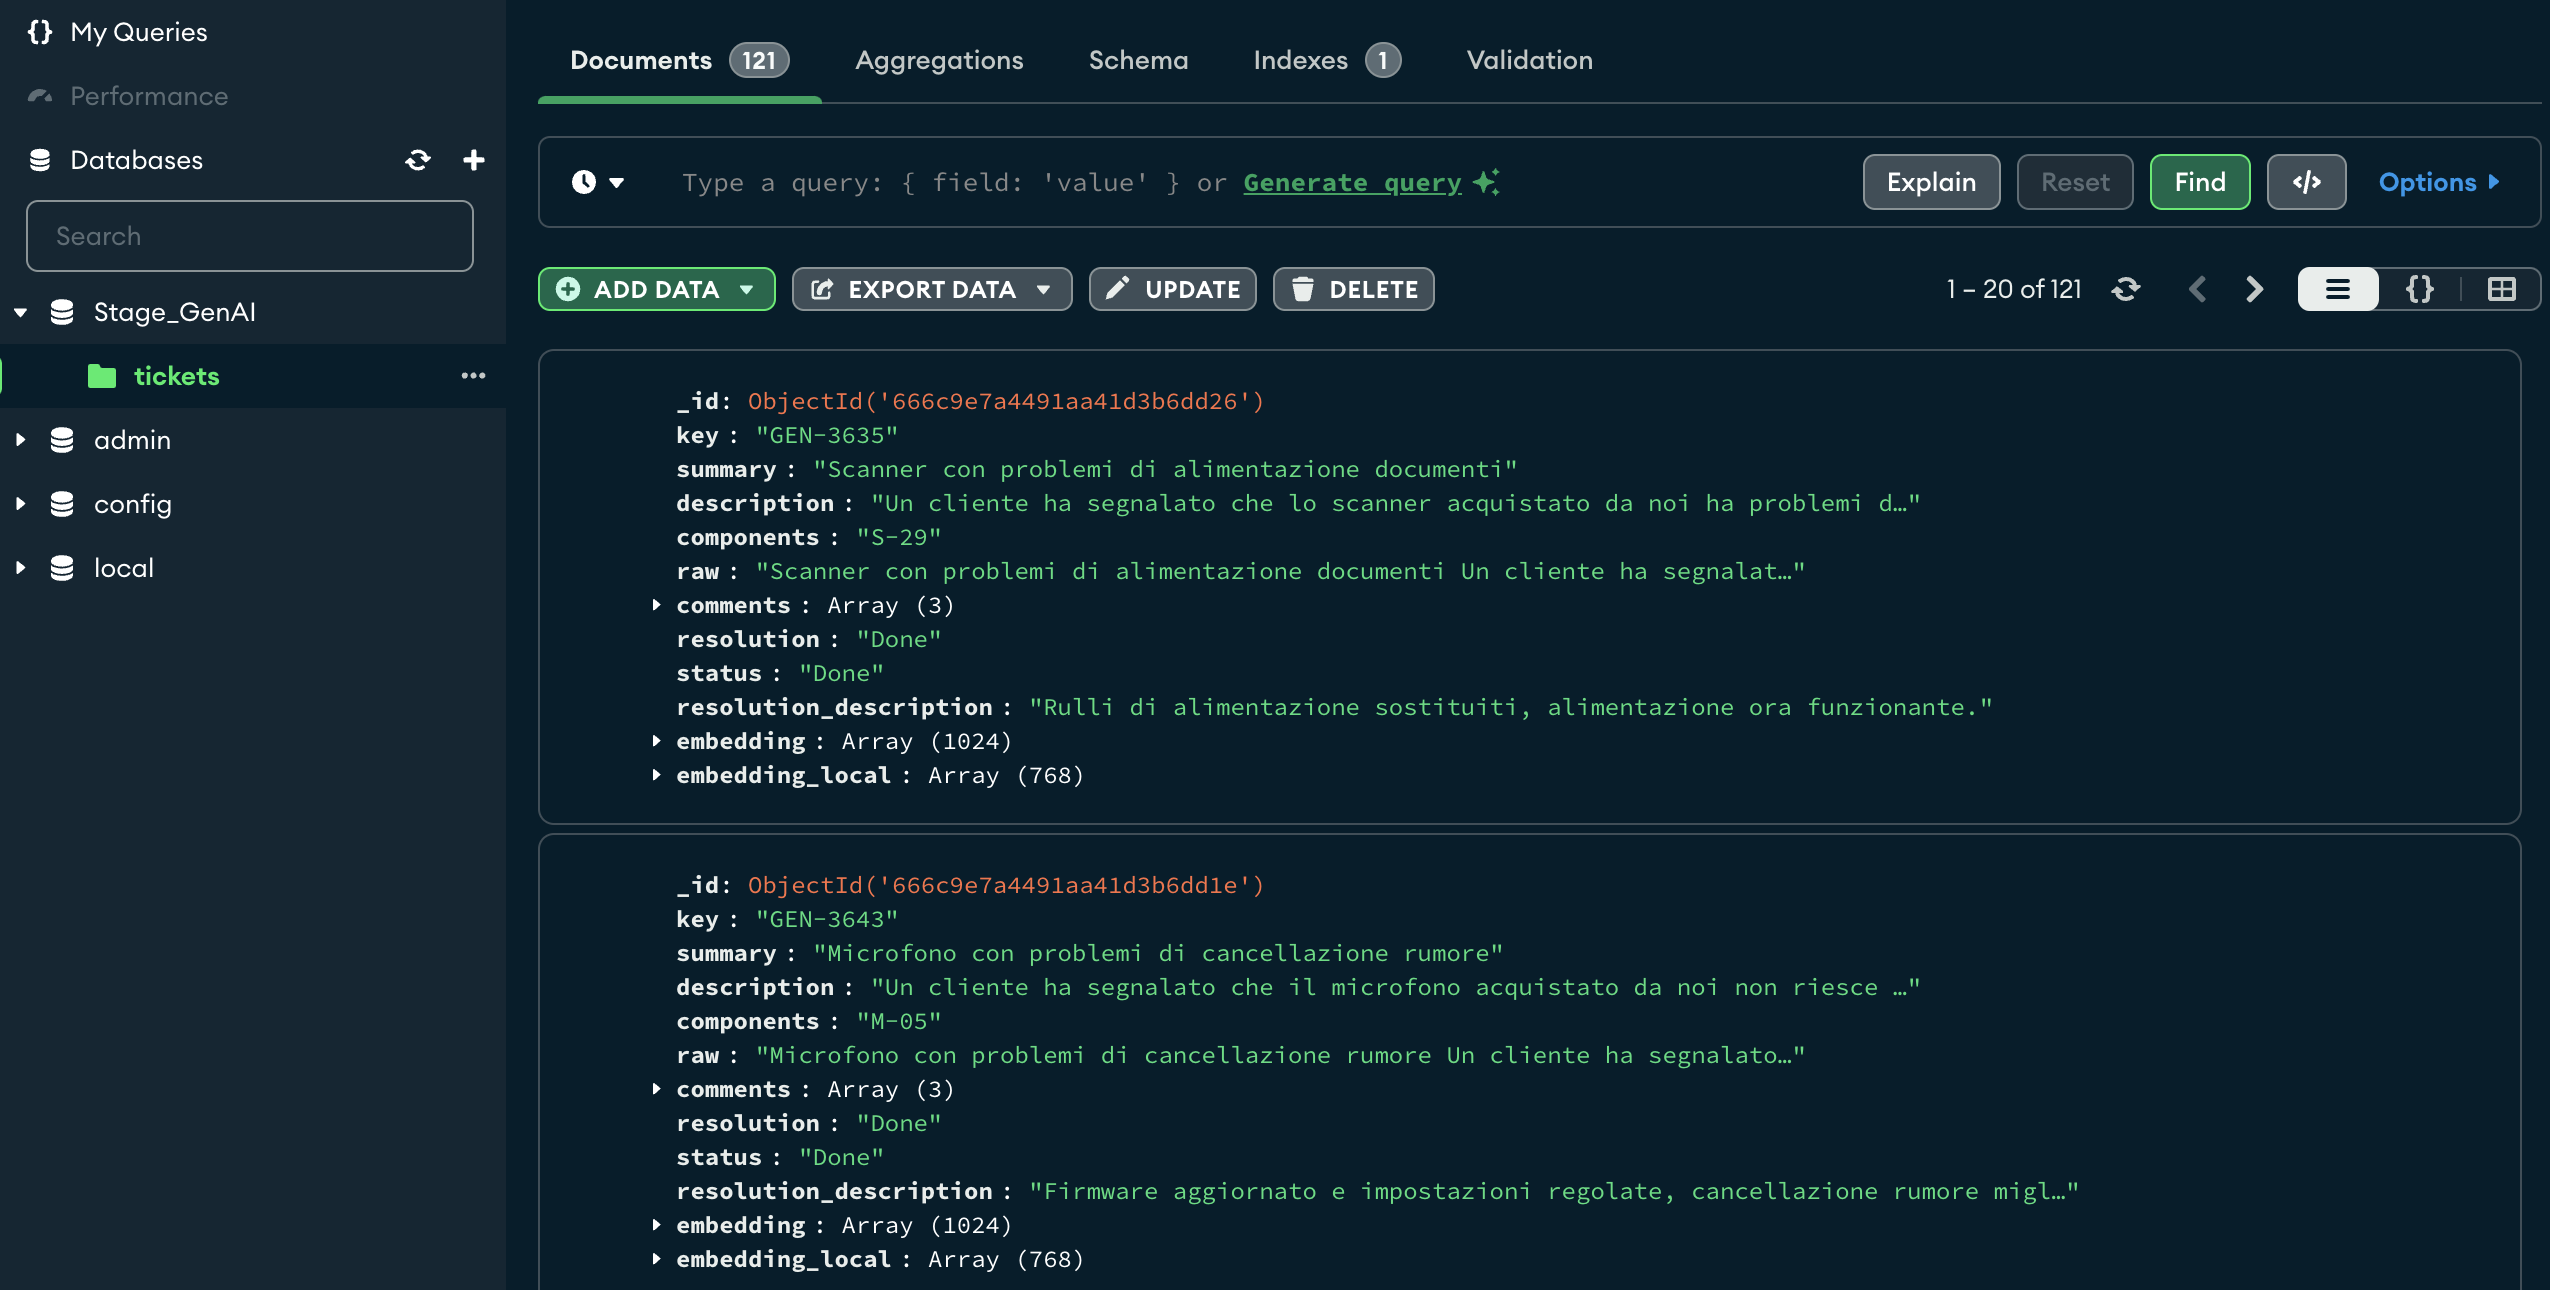
\includegraphics[width=0.85\textwidth]{mongodb.png}
    \caption{Esempio di visualizzazione di documenti su MongoDB Compass}
    \label{fig:MongoDB}
\end{figure} 
%\noindent Esempio di utilizzo di un termine nel glossario \\
%\gls{api}. \\

%\noindent Esempio di citazione in linea \\
%\cite{site:Agile-manifesto}.

%\noindent Esempio di citazione nel pie' di pagina \\
%citazione\footcite{womak:lean-thinking} \\
\noindent
Di seguito uno schema riassuntivo in cui mostro l'utilizzo delle tecnologie nel progetto di \textit{stage}.
\begin{figure}[H]
    \centering
    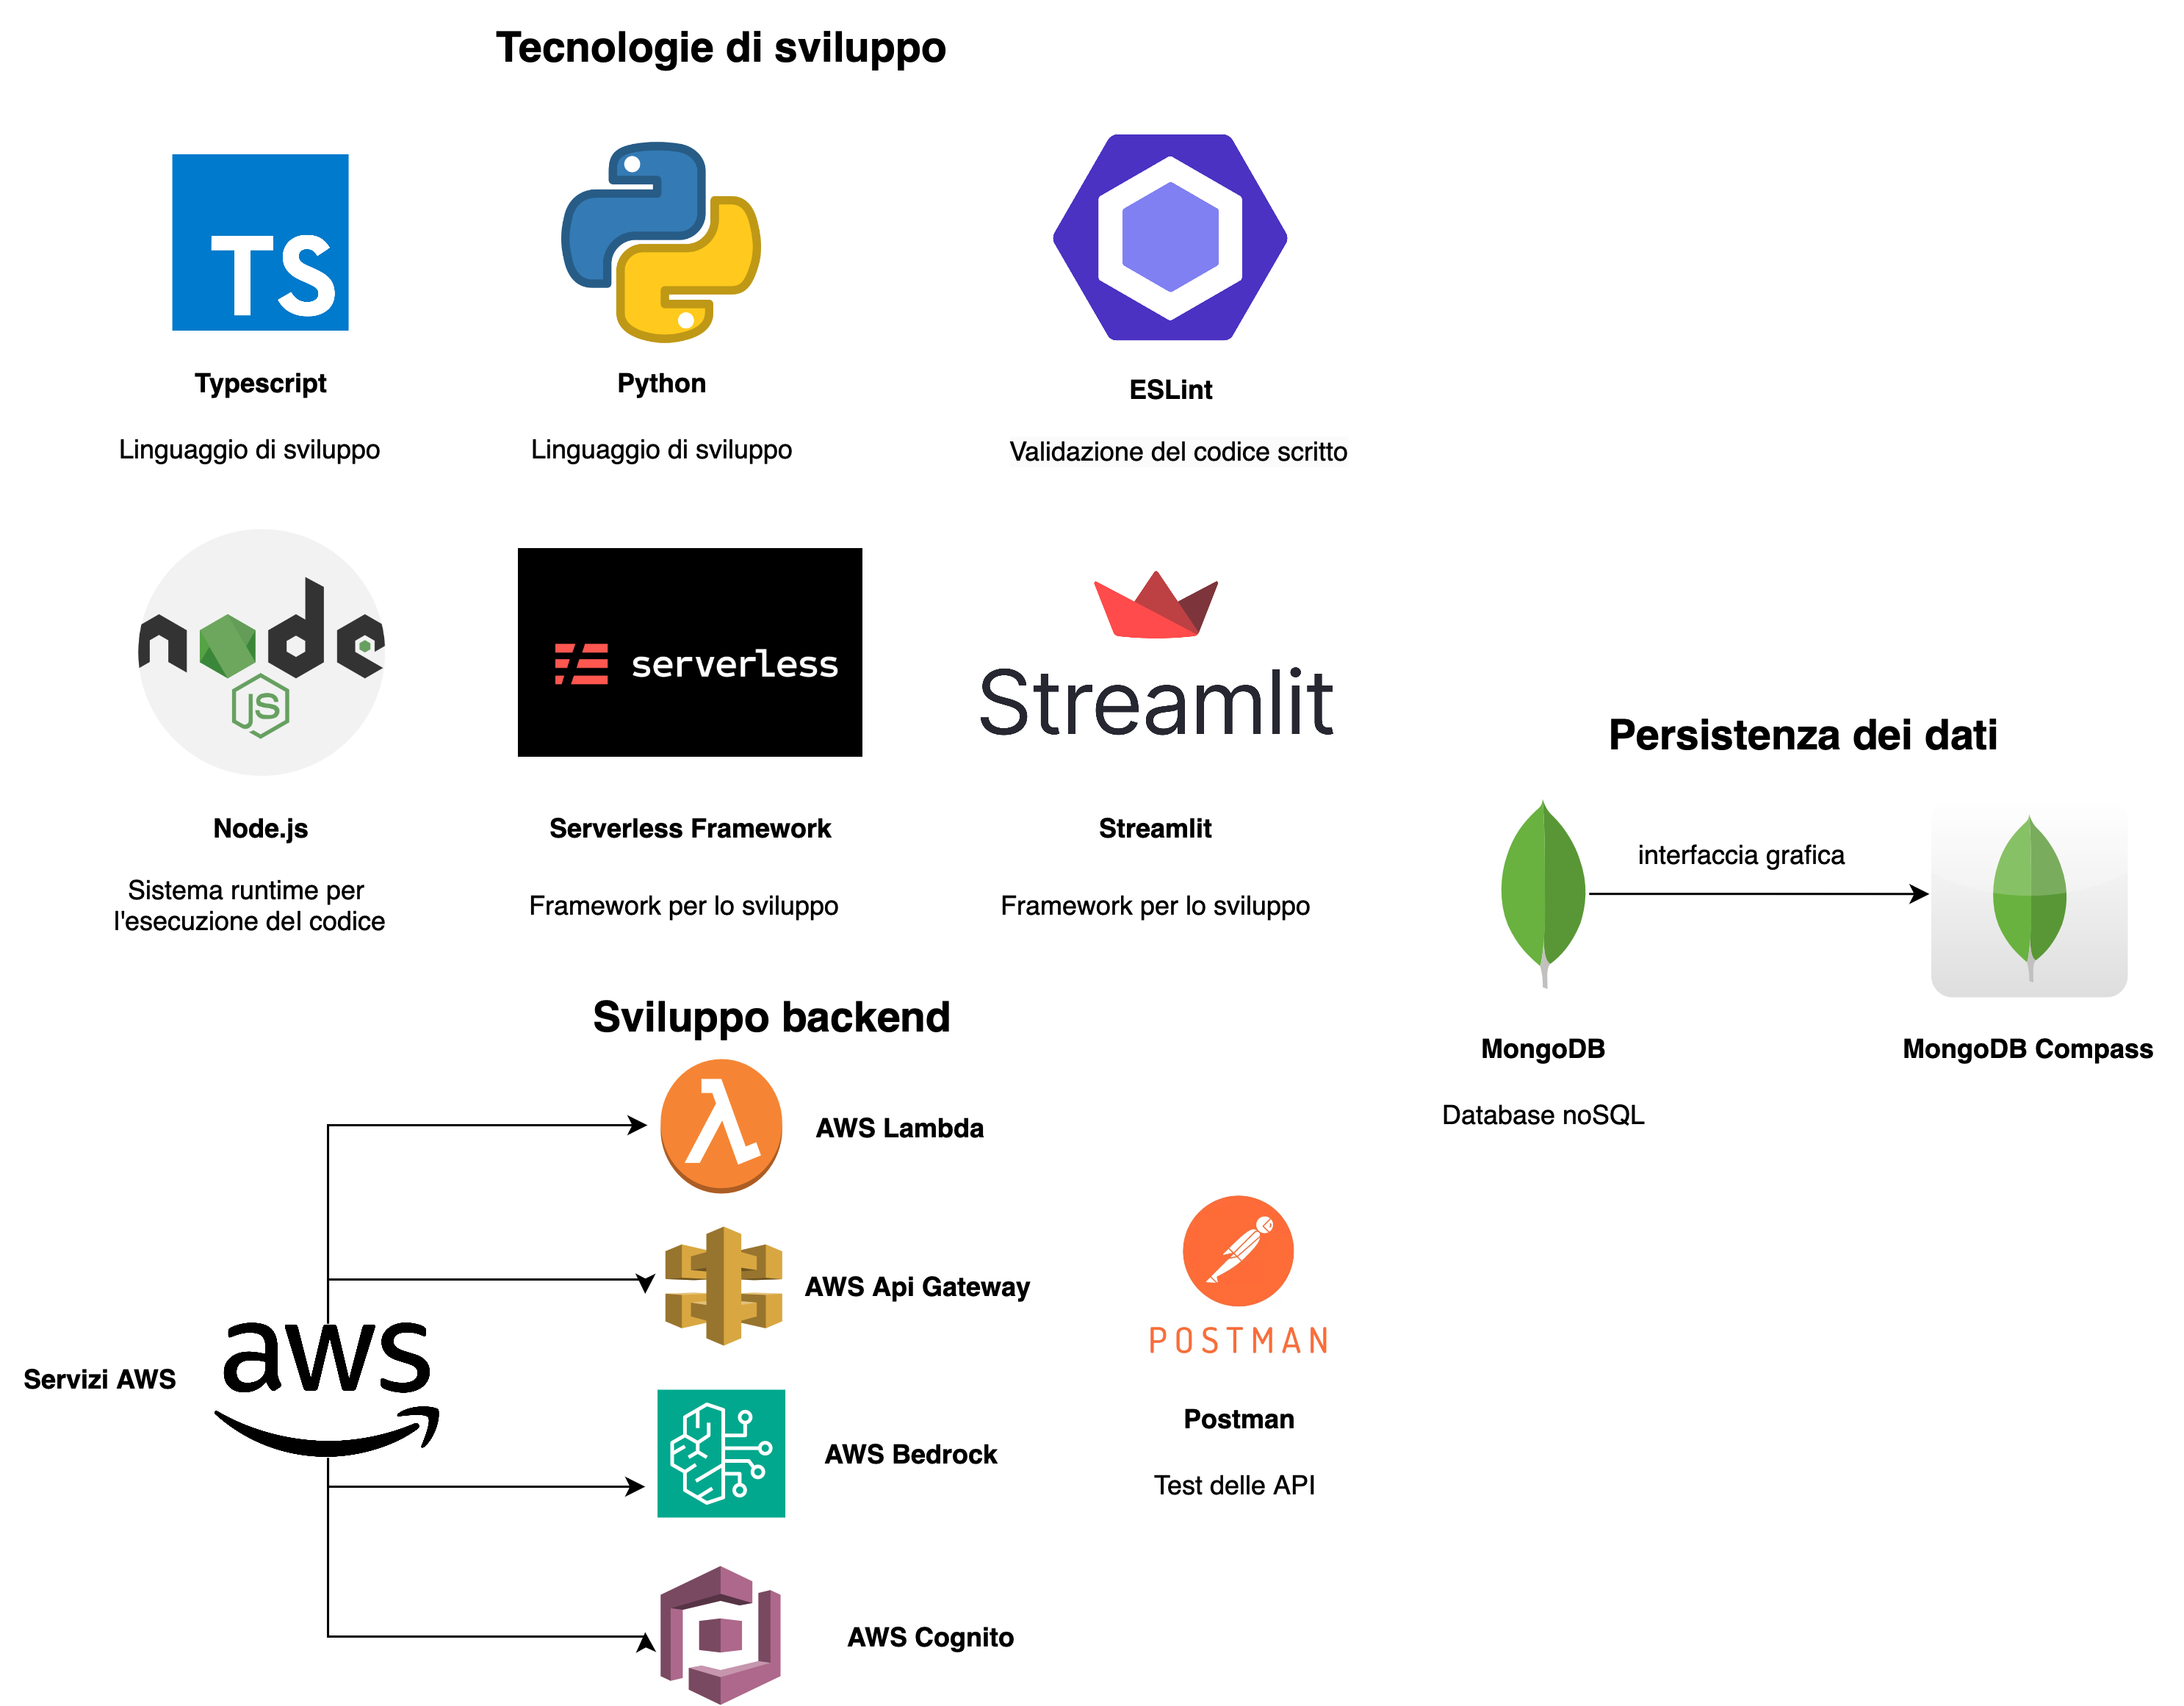
\includegraphics[width=1\textwidth]{tecnologie.png}
    \caption{Utilizzo delle tecnologie nel progetto di \textit{stage}}
    \label{fig:tecnologie}
    \small \textbf{Fonti:} \href{https://iconduck.com/icons/95017/typescript-icon}{Typescript: https://iconduck.com} \href{https://www.flaticon.com/free-icon/nodejs_919825}{Node\.js: https://www.flaticon.com} \href{https://www.iconfinder.com/icons/4518857/python_icon} {Python: https://www.iconfinder.com} \href{https://iconduck.com/icons/94274/eslint} {Eslint: https://iconduck.com} \href{https://www.serverless.com/} {Serverless: https://www.serverless.com} \href{https://iconduck.com/icons/10826/amazon-aws} {AWS: https://iconduck.com} \href{https://www.nuget.org/packages/LangChain/0.13.1-dev.178} {Langchain: https://www.nuget.org} 
\end{figure}
\section{Tipologia di clientela} \label{sec:clientela}
Durante il mio periodo di \textit{stage} , ho avuto modo di osservare la diversità dei clienti che si rivolgono a Zero12 s.r.l. Tra i committenti dei vari progetti sviluppati dall'azienda, ci sono numerose aziende operanti nel medesimo settore, le quali richiedono consulenze sulle tecnologie di cui l'azienda è \textit{partner}.
L'azienda collabora anche con clienti provenienti da settori diversi, come ad esempio il settore della moda, con \textit{brand} di lusso che richiedono lo sviluppo di software \textit{custom} per la gestione dei propri prodotti o servizi.

\section{Propensione all'innovazione}
L'azienda è fortemente orientata all'innovazione e alla sperimentazione di nuove tecnologie.
L'azienda si propone ai suoi nuovi clienti come \textit{Innovation advisor} riuscendo a sviluppare soluzioni innovative in linea con le esigenze del cliente. Essendo \textit{parter} \gls{aws}, l'azienda è particolarmente incentrata nella ricerca di innovazione in ambito \textit{cloud}.
In aggiunta, l'azienda organizza eventi interni per discutere o assistere alla presentazione di nuove tecnologie, portando cosi nuove idee anche non inerenti all'ambito \textit{cloud}. Un esempio, è stato la partecipazione collettiva in sede aziendale, all'evento annuale Apple \textit{Worldwide Developers Conference} organizzato da Apple. In questa occasione, i presenti hanno assistito alla presentazione delle nuove funzionalità presentate e discusso le loro possibili applicazioni in progetti futuri.

%\section{Organizzazione del testo}

%\begin{description}
    %\item[{\hyperref[cap:introduzione]{Il primo capitolo}}] descrive ...
    %\item[{\hyperref[cap:lo-stage]{Il secondo capitolo}}] descrive ...
    
    %\item[{\hyperref[cap:descrizione-stage]{Il terzo capitolo}}] approfondisce ...
    
    %\item[{\hyperref[cap:conclusioni]{Il quarto capitolo}}] approfondisce ...
    
%\end{description}

%Riguardo la stesura del testo, relativamente al documento sono state adottate le seguenti convenzioni tipografiche:
%\begin{itemize}
	%\item gli acronimi, le abbreviazioni e i termini ambigui o di uso non comune menzionati vengono definiti nel glossario, situato alla fine del presente documento;
	%\item per la prima occorrenza dei termini riportati nel glossario viene utilizzata la seguente nomenclatura: \emph{parola}\glsfirstoccur;
	%\item i termini in lingua straniera o facenti parti del gergo tecnico sono evidenziati con il carattere \emph{corsivo}.
%\end{itemize}
